\documentclass[sigconf,nonacm,10pt]{acmart}
\settopmatter{printacmref=false, printfolios=false}
\pagestyle{plain}
\usepackage{graphicx}
\usepackage{booktabs}
\usepackage{amsmath}
\usepackage{siunitx}
\usepackage{xeCJK}
\setCJKmainfont{STSong}
\setCJKsansfont{STHeiti}
\setCJKmonofont{STFangsong}
\emergencystretch=3em
\tolerance=1200
\hbadness=10000
\graphicspath{{../figs/}}
\newcommand{\SolEth}{SOL$\to$ETH}
\newcommand{\EthSol}{ETH$\to$SOL}
\newcommand{\gsigned}{g_{\text{signed}}}
\newcommand{\Cexec}{C_{\text{exec}}}
\newcommand{\Rgross}{R_{\text{gross}}}
\title{第四章 --- Solana 与 EVM 间的跨链 MEV：基于 Wormhole Portal 的端到端实证框架}
\author{匿名}
\affiliation{\institution{-}\country{-}}
\begin{document}
\maketitle



\section{为何选择 Wormhole Portal，以及数据集的构造}
\label{sec:ch4-data}

\subsection{为何选择 Wormhole Portal？}

当前承载 Solana$\leftrightarrow$Ethereum 跨链流量的通用桥主要有五条：
Relay、Mayan Finance、Chainlink CCIP、LayerZero~V2 与 Wormhole Portal。
本研究以 Wormhole 作为唯一的研究对象，原因如下五点彼此交织、互为支撑。

\begin{enumerate}
    \item \textbf{历史最长、流量最深。} 作为两个生态间最早的开放许可制
        通用消息层，Portal 拥有最长的连续事件记录（\texttt{/operations}
        API 可一直回溯至上线初期）；同时，在五条桥中，它日均承载的
        SOL$\leftrightarrow$ETH 资产转移流量最大，能为长达 $365$ 天的
        实证研究提供足够的统计功效。
    \item \textbf{基于 VAA 的链上可直接核验。} Wormhole 的每一条消息都由
        Guardian 集群以密码学签名背书，并以 \emph{Verifiable Action
        Approval}（VAA）形式落链。这使得我们可以\emph{无需}任何链下台账，
        仅凭密码学证据将一笔 Solana 签名同对应的 Ethereum 交易哈希一一
        匹配，是后续跨链 PnL 重建不可或缺的前提。
    \item \textbf{标准化的双端配对模式。} Portal 在两条链上的 Token
        Bridge 合约采用固定的 emitter/recipient 字段结构，因此对于每一
        条记录，发款方与收款方都能被统一解码。这一性质使得我们能够构造
        $(sol\_addr, eth\_addr)$ 这一“行为者”关键字，所有集中度、往返、
        行为者特征分析均建立在其之上。
    \item \textbf{传输与执行天然解耦。} 桥本身只完成转账原语；任何随后
        的 DEX 执行都属于独立的链上事件，并具有独立的日志。这使得我们
        能够将一次跨链套利的三个子过程---\emph{入场 swap、桥腿、出场
        swap}---相互解耦，而不会与桥的内部记账纠缠。
    \item \textbf{代币覆盖与实际套利样本一致。} 实际观察到的跨链套利
        几乎完全由长尾 memecoin 驱动；Wormhole（通过 WTT 与 NTT 两套
        标准）在该细分市场中所支持的代币集合是其余四条桥的真超集，因
        此“仅采集 Wormhole”不会对所研究的现象造成显著的样本选择偏差。
\end{enumerate}

\subsection{数据采集流水线}
\label{sec:ch4-pipeline}

我们按以下五个阶段顺序采集数据（图~\ref{fig:ch4-pipeline}）。该流水线
原始体量颇大：候选套利记录约 $30{,}729$ 条、附带上下文的匹配 JSON 约
$292$~MB、Ethereum 端 1 分钟价格序列按代币拆分后共约 $804$~MB。由于反
复在内存中解析这些数据曾在测试机上触发 OS 级别的内存失败，本流水线后
续被重新设计为模块级单例缓存 + 按代币分片（$165$ 个 LRU 文件）+
预测子流水线 5 处磁盘检查点的混合架构，最终能在 $<2$~GB 常驻内存内端
到端运行完毕。

\clearpage
\begin{figure*}[!t]
    \centering
    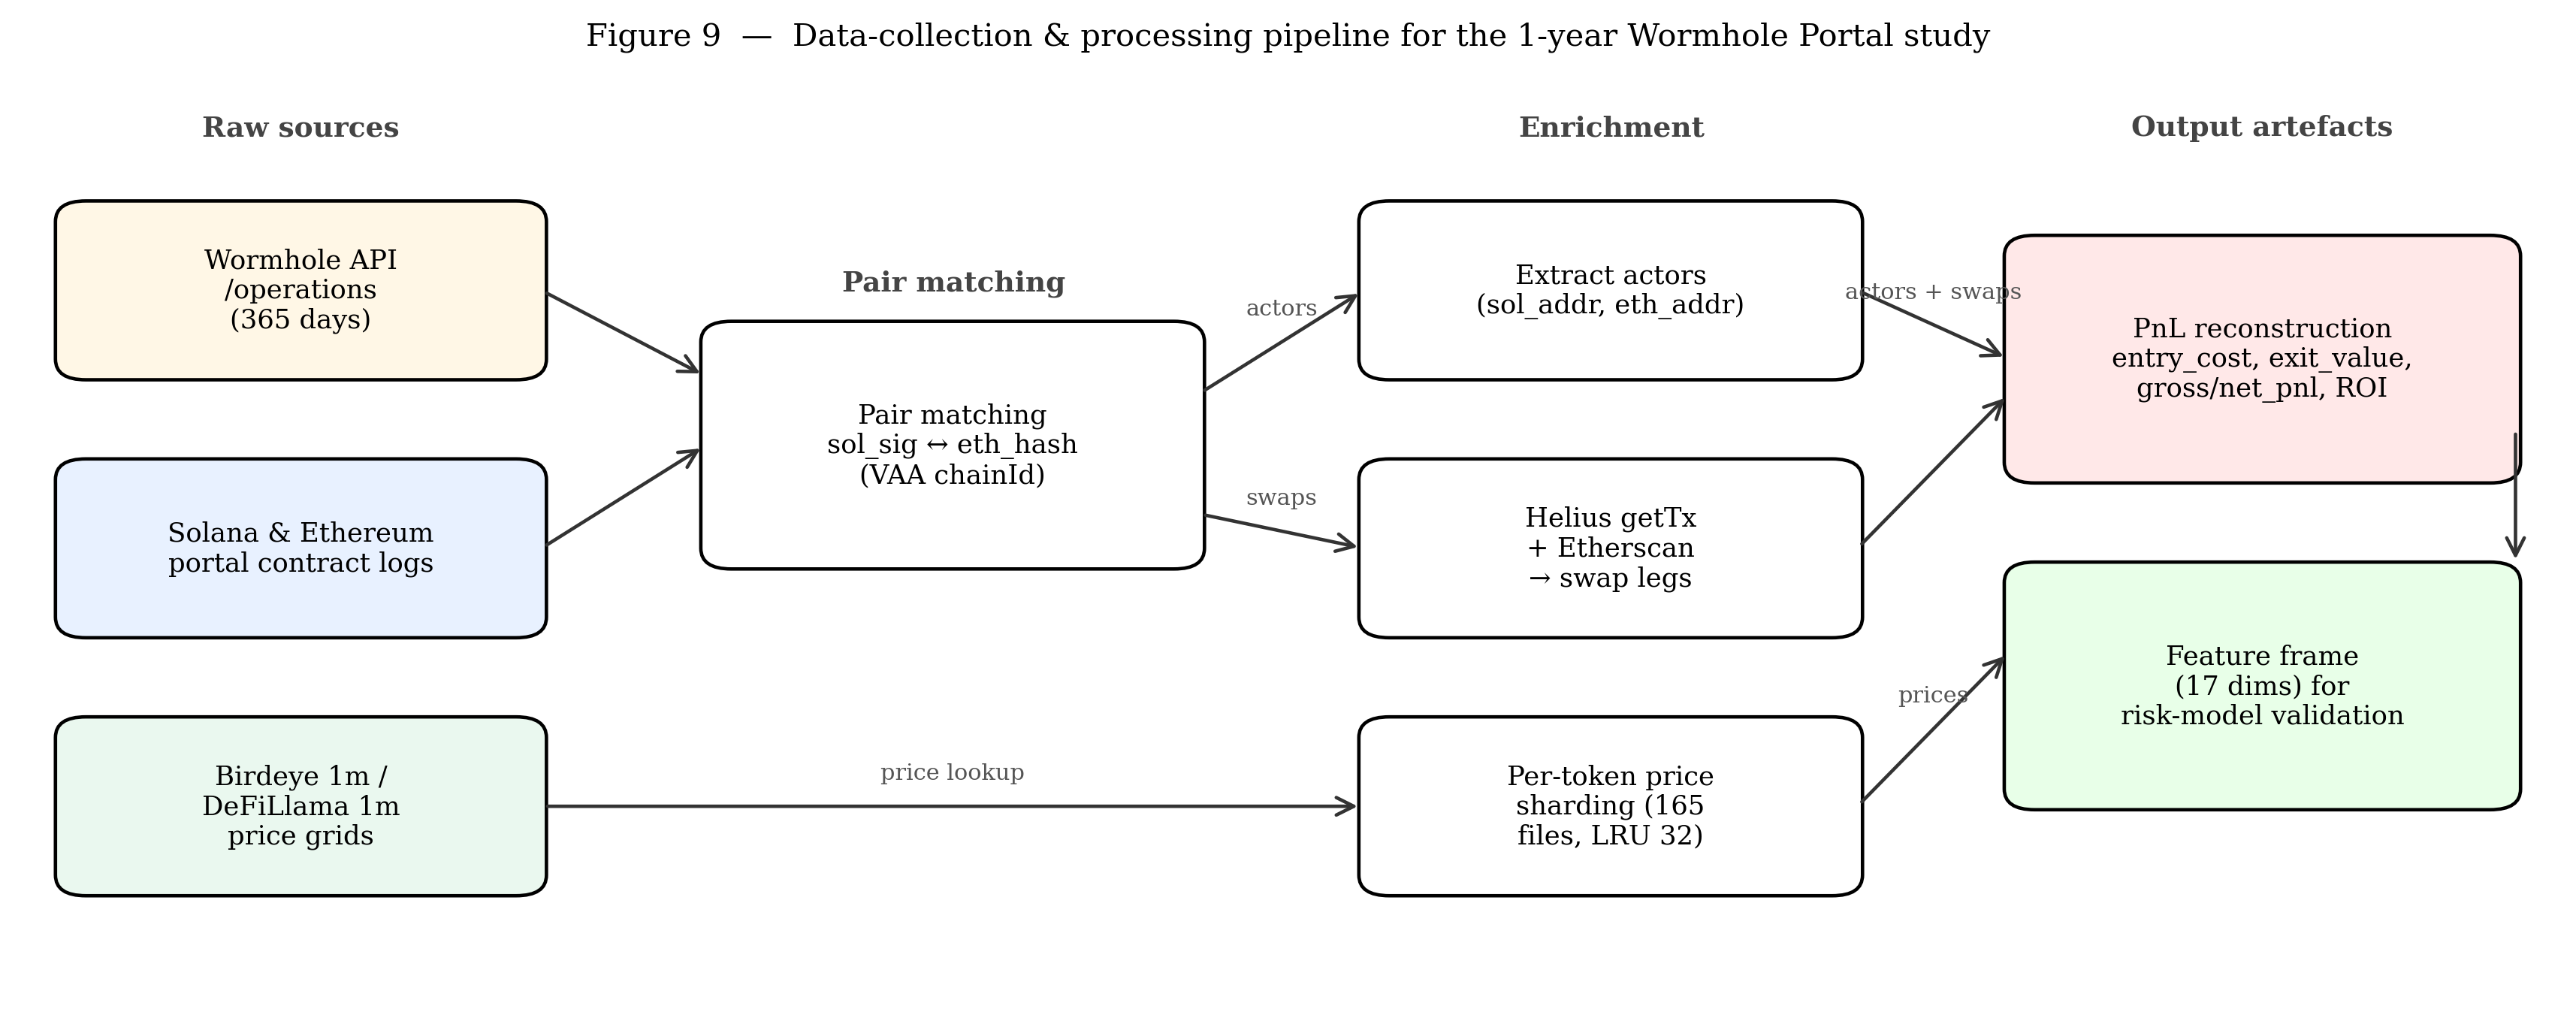
\includegraphics[width=0.98\textwidth]{09_pipeline.png}
    \caption{Wormhole Portal 一年期研究的数据采集与处理流水线。}
    \label{fig:ch4-pipeline}
\end{figure*}

\paragraph{图~\ref{fig:ch4-pipeline} 逐块解读。} 示意图由左至右
分为 \emph{四个}带标签的阶段。\textbf{阶段~1（Raw sources）}是
最左侧一列的三个彩色框：Wormhole \texttt{/operations} API（黄）、
Solana/Ethereum Portal 合约日志（蓝）、Birdeye/DeFiLlama 1~分钟
价格网格（绿）。\textbf{阶段~2（Pair matching）}是中间单一的
配对框，以 VAA 链 ID~+~sequence number 把两条链上各自的签名流
合并为一条跨链记录，形成 4 元组 $(\texttt{direction},\allowbreak\
\texttt{sol\allowbreak\_sig},\allowbreak\ \texttt{eth\allowbreak\_sig},
\allowbreak\ \texttt{eth\allowbreak\_hash})$。\textbf{阶段~3
（Enrichment）}是一列三个框：提取套利行为者
\texttt{(sol\allowbreak\_addr,\ eth\allowbreak\_addr)}、通过
Helius \texttt{getTx} + Etherscan 补齐 swap 腿、并从 165 文件
分片 LRU 缓存拉取每代币价格。\textbf{阶段~4（Output
artefacts）}是最右侧两个框：上方为重构后的 PnL 账本
（\texttt{entry\allowbreak\_cost}、
\texttt{exit\allowbreak\_value}、
\texttt{gross/net\allowbreak\_pnl}、ROI），下方为下游风险模型
验证所使用的 17 维特征矩阵。阶段之间的箭头带有明确标签
（\emph{price lookup}、\emph{actors}、\emph{swaps}、\emph{prices}）。
注意：研究样本的漏斗宽度（$30{,}729\to 28{,}574\to 28{,}554$）
在下文正文中报告，\emph{并未}直接在图上标注。

\paragraph{阶段~1 --- 原始数据源。} 在 2025-04-15~---~2026-04-14（共
$364$ 天）窗口内，我们并行查询三类原始来源：
(i) Wormhole \texttt{/operations} API，枚举所有
SOL$\leftrightarrow$ETH 消息；
(ii) 通过 Helius RPC 的 \texttt{getSignaturesForAddress} 抓取 Solana
端 Portal 合约日志；
(iii) 通过 Etherscan 与直接 RPC 抓取 Ethereum 端 Portal 合约日志。
与此同时，我们从 Birdeye 预取 Solana 端代币的 1 分钟价格网格，从
DeFiLlama 预取 Ethereum 端代币的对应价格网格。

\paragraph{阶段~2 --- 配对匹配。} 每条 Wormhole 消息均带有 VAA 链 ID
与序列号，可唯一定位另一条链上的对应腿。我们以此将每一条源端签名
\texttt{sol\_sig} 与目的端哈希 \texttt{eth\_hash} 一对一配对（反向同
理）。该匹配是\emph{纯密码学}的，不依赖任何时间窗启发式。匹配后，每条
记录均带有四元组
$(\texttt{direction, sol\_sig, eth\_sig, eth\_hash})$ 以及双端的
Wormhole 出账金额。

\paragraph{阶段~3 --- 行为者抽取与上下文增强。} 对每条匹配记录，我们解
码两端的 signer/payer 字段，得到两个行为者属性：\texttt{arb\_sol}
（Solana base58 公钥）与 \texttt{arb\_eth}（Ethereum 十六进制地址）。
将其在所有记录上取并集后，得到一个全局行为者集合，共 $321$ 个独立的
$(sol\_addr, eth\_addr)$ 配对。对其中每一个行为者，我们再分别在两条链
上拉取其完整的 1 年交易历史，使得每一条候选事件都能被嵌入到“行为者本
地的 DEX 活动上下文”中：在桥腿前后某可配置时间窗（典型为 $\pm 60$ 秒）
内，行为者钱包上发生的所有 swap 都会作为
\texttt{entry\_swaps\_greedy} 与 \texttt{exit\_swaps\_greedy} 被抽出。
正是这一步把\emph{桥转账}与\emph{跨链套利}区分开来：后者要求两端均存
在临近的 DEX swap。

\paragraph{阶段~4 --- PnL 重建。} 对每条候选事件，我们计算：
\begin{itemize}
    \item $\Cexec^{\text{in}}$：入场腿的实际美元成本---由每个输入代币
        的数量乘以其在 \texttt{sol\_ts}（或 \texttt{eth\_ts}）时刻的
        每分钟价格构成；
    \item $V^{\text{out}}$：出场腿的实际美元价值---由出场端代币在出场
        时刻的价格估算；
    \item $\Pi_{\text{gross}} = V^{\text{out}} - \Cexec^{\text{in}}$；
    \item $\Pi_{\text{net}} = \Pi_{\text{gross}} - f_{\text{sol}} - f_{\text{eth}}$，
        即扣除两端实际 gas 费用后的净 PnL。
\end{itemize}
\paragraph{Dust 入场工件过滤。} 在进入任何后续分析之前，我们先剔除
$\Cexec^{\text{in}}<\$1$ 的候选 —— 此阈值低于链上交易的最低可行成本
（以太坊 L1 上一笔 swap 仅 gas 就需 \$1--\$5）。这些样本是 pipeline
工件：桥接包装环节的 token 金额舍入会把
$\mathrm{ROI}=\Pi_{\text{net}}/\Cexec^{\text{in}}$ 的分母压到接近零，
从而生成高达 $10^{11}\%$ 的荒谬数值（最极端的 5 笔全部是 \EthSol{}
方向的 TRUMP，$\Cexec^{\text{in}}<\!10^{-5}$\,USD 而 PnL 为几百美金）。
该过滤共剔除 11 笔（$0.04\%$）；我们**刻意不**以"手续费 $>$ 入场"为
过滤条件，因为这属于真实经济亏损而非测量误差。经此步骤后候选样本
共 $30{,}729$ 条。

我们再为每条事件赋予一个可靠性标签
\texttt{pnl\_reliability}~$\in$~\{reliable, \allowbreak reliable\allowbreak\_after\allowbreak\_dedup\allowbreak\_failed, \allowbreak unreliable\allowbreak\_asymmetric, \allowbreak unreliable\allowbreak\_partial\allowbreak\_holdings\}，依据是双端腿
覆盖一致性的若干健康检查。本研究在所有后续分析中只使用 \texttt{reliable}
等级（$N=28{,}574$，占候选样本的 $93.0\%$），并进一步剔除该等级内
PnL 最极端的 20 笔事件（最大亏损 Top-10 与最大盈利 Top-10，合计
占可靠样本 $<\!0.07\%$）---这些事件的 PnL 实为定价流水线在近乎空
池上产生的假象（例如
\texttt{dead\allowbreak\_pool\allowbreak\_exploit} /
\texttt{thin\allowbreak\_pool\allowbreak\_arb} 上的 wrapped 资产事件，
SOL 侧流动性 $\leq\!\$25$\,k 却承接 $\geq\!\$10$\,k 的名义仓位）。
最终研究样本为 $N = 28{,}554$。

\paragraph{阶段~5 --- 特征矩阵。} 将可靠子集与流动性属性
（\texttt{sol\_liq\_usd, eth\_liq\_usd}）、24 小时成交量代理、市值估
计以及带符号的入场价差
\begin{equation}
\label{eq:ch4-gsigned}
    \gsigned = \mathrm{sign}_{\text{dir}}\!\cdot\!
    \bigl(P_{\text{dst}}/P_{\text{src}}-1\bigr)\!\times\!100\%,
\end{equation}
（基于所桥接代币在两端入场时刻的价格）拼接，得到一个 17 维的特征矩
阵，作为下游所有分析的输入。

\section{跨链套利：定义与实证画像}
\label{sec:ch4-arbitrage}

\subsection{定义}

在本章中，所谓\emph{跨链套利事件}的结构定义如下。

\begin{quote}
\textbf{定义 1（跨链套利）。} 一个观测 $e$ 称为\textit{跨链套利事件}，
当且仅当其由三段因果相连的链上腿构成
\[
    L_{\text{entry}} \;\to\; L_{\text{bridge}} \;\to\; L_{\text{exit}}
\]
且满足：(i) $L_{\text{entry}}$ 与 $L_{\text{exit}}$ 各自至少包含一笔
DEX swap，且分布于两条不同的链；(ii) $L_{\text{bridge}}$ 所转移的资
产与金额，与 $L_{\text{entry}}$ 的输出和 $L_{\text{exit}}$ 的输入相
洽；(iii) 三段腿共享同一个 $(sol\_addr, eth\_addr)$ 行为者。
\end{quote}

我们\emph{不}要求 $\Pi_{\text{net}} > 0$：本研究关心的是套利的\emph{
意图}与\emph{结构}，而不是其事后是否成功。我们也\emph{不}要求
$\gsigned$ 超过某阈值：任何被观测到的跨链价差，无论其成因如何，都构
成一个套利信号\footnote{在数据采集前置阶段我们设置了 10\% 的价差上限
以约束样本体量；本研究后续所有分析均不再施加任何价差阈值，使用全部
\texttt{reliable} 子集。}。这与本研究先前所确立的方法论原则一致：
``任何跨链价差皆为套利；价差成因与执行速度均不能作为有效性判据''。

\subsection{实证画像}
\label{sec:ch4-empirical}

图~\ref{fig:ch4-macro}--\ref{fig:ch4-model} 给出了 Wormhole 上可靠跨
链套利的一年期实证画像。

\clearpage
\begin{figure*}[!t]
    \centering
    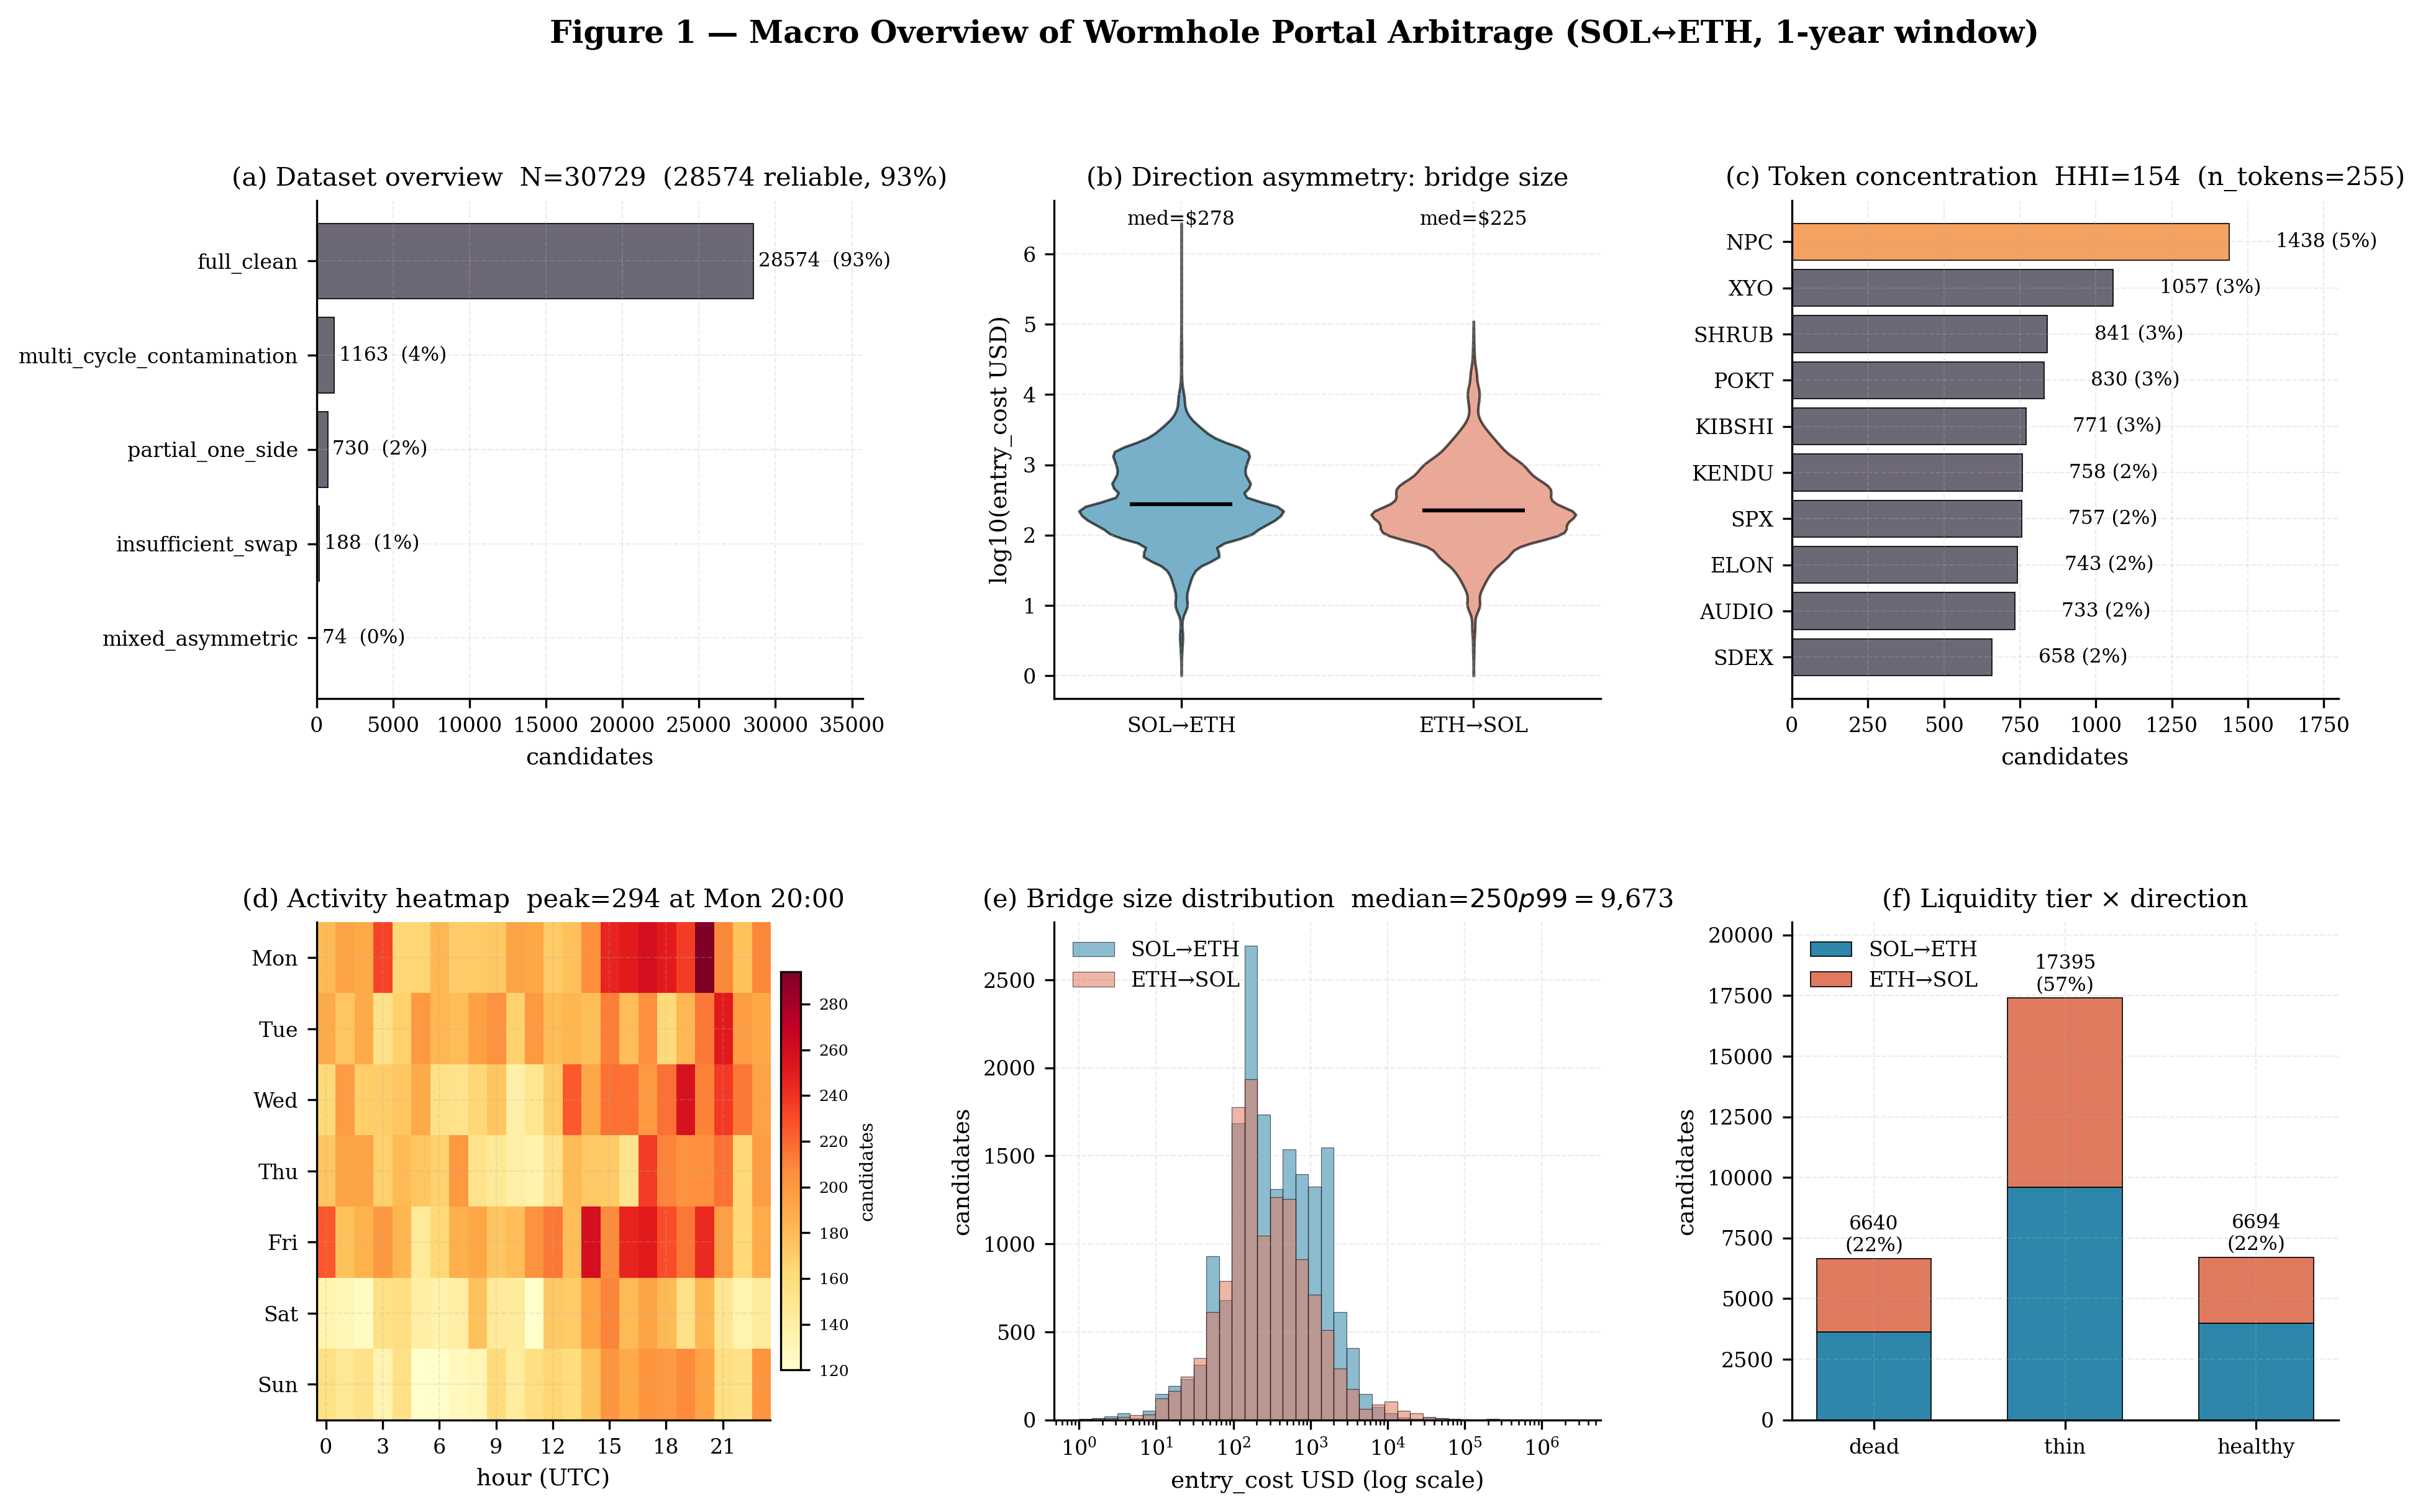
\includegraphics[width=0.99\textwidth]{01_macro.png}
    \caption{宏观结构：数据漏斗 (a)、按方向对数规模分布 (b)、Top-15
    代币 Herfindahl 条形图 (c)、UTC 小时~$\times$~星期活跃度热图 (d)、
    整体规模直方图 (e) 与流动性分层~$\times$~方向堆叠柱 (f)。}
    \label{fig:ch4-macro}
\end{figure*}

\paragraph{图~\ref{fig:ch4-macro} 逐块解读。} 面板~(a) 为按
\texttt{subtype} 对所有候选记录统计的水平条形图；图标题直接
标注 $N=30{,}729$ 总数与 $n_{\text{rel}}=28{,}574$ 可靠
（$93\%$），汇总了上游流水线漏斗，后续再剔除 20 笔极端尾部
事件得到研究样本 $N=28{,}554$。面板~(b) 将按方向计算的入场
规模取 $\log_{10}$ 并以并列小提琴图呈现；两个方向在中位数附近
（\SolEth{} 为 \$268，\EthSol{} 为 \$200）高度重合，但 \SolEth{}
右尾明显更长。面板~(c) 以水平条形图列出 Top-10 最活跃的代币，
并在条末附上绝对数与占比标签；图标题中的代币层 Herfindahl
指数仅 $665$，最底部（高亮）那根柱对应成交次数最多的单一代币。面板~(d) 为星期~$\times$~
UTC 小时热图：流量在美洲下午时段（16--22~UTC）达到峰值。面板~(e)
是整体桥接规模在对数横轴上的直方图，分布呈对数正态，峰值集中
于 \$200--\$300 的狭窄区间。面板~(f) 为 (流动性分层~$\times$~
方向) 的堆叠柱图：\texttt{thin\allowbreak\_pool\allowbreak\_arb}
占主导（约 $16$\,k 条事件），其次为
\texttt{dead\allowbreak\_pool\allowbreak\_exploit} 与
\texttt{healthy\allowbreak\_market\allowbreak\_arb}，各约 $6$\,k 条
——本章后文所要解读的正是这一“流动性地貌”。

\clearpage
\begin{figure*}[!t]
    \centering
    
\includegraphics[width=0.99\textwidth]{02_timing.png}
    \caption{时间结构：按方向的桥接延迟 CDF (a)、原子性矩阵 (b)、
    桥与 swap 间隔 (c)、按延迟档位的 ROI (d)。}
    \label{fig:ch4-timing}
\end{figure*}

\paragraph{图~\ref{fig:ch4-timing} 逐块解读。} 面板~(a) 在对数横轴
上绘制桥接延迟 $|\Delta t|$ 的 CDF：\SolEth{} 几乎垂直收敛至
$34$\,s 的平台，而 \EthSol{} 直到 $10^{3}$\,s 以上才开始趋于
平台——这是以太坊终局性驱动的 $\approx\!30\times$ 延迟不对称的
直接视觉证据。面板~(b) 为 (入场同区块)~$\times$~(出场同区块) 的
$2\!\times\!2$ 原子性矩阵；只有 $28$ 笔事件（$0.10\%$）落入完全
原子的格子。面板~(c) 分别针对入场与出场 swap 绘制
$|t_{\text{swap}} - t_{\text{bridge}}|$ 的直方图：众数均在 $10$
至 $10^{2}$\,s 之间，但出场 swap 的分布右尾更肥。面板~(d) 按
桥接延迟档位分箱并以每档箱线图呈现 ROI：反直觉地，最慢档位
的 ROI 中位数\emph{最高}（约 $2$--$3\%$），最快档位反而跌至
约 $0.5\%$，这是第~\ref{sec:ch4-refined-model} 节“平台叠加
指数”型 $\phi(\Delta)$ 拟合的视觉前兆。

\clearpage
\begin{figure*}[!t]
    \centering
    
\includegraphics[width=0.99\textwidth]{03_economics.png}
    \caption{经济性：ROI 直方图及 CDF 子图 (a)、按方向 ROI CDF (b)、
    资本档位分布 (c)、手续费负担比 (d)、毛~$\to$~净 PnL 散点 (e)，
    以及资本~$\to$~净 PnL 回归 (f)。}
    \label{fig:ch4-econ}
\end{figure*}

\paragraph{图~\ref{fig:ch4-econ} 逐块解读。} 面板~(a) 为截至
$\pm 20\%$ 的 ROI 直方图，并在 $\pm 10\%$ 范围内嵌入放大 CDF 子图；
整体呈强右偏分布。面板~(b) 将两个方向的 ROI CDF 叠加：\EthSol{}
的中位数略高（$1.61\%$），但 \SolEth{} 的上尾更重。面板~(c) 将
\texttt{entry\allowbreak\_cost} 划分为十进制档位并绘制每档计数条：
绝大多数活动（约 $17$\,k 条事件）处于 \$100--\$1\,k 档，\$10\,k
以上仅约 $137$ 条。面板~(d) 在对数横轴上绘制手续费负担比
$f_{\text{total}} / |\Pi_{\text{gross}}|$；中位数远低于 $0.1$，
表明 gas 非主导成本。面板~(e) 为 $\Pi_{\text{gross}}$ 与
$\Pi_{\text{net}}$ 的散点图，点几乎全部落在 45° 线上或略偏下。
面板~(f) 为剔除 20 笔极端事件后资本$\to$净 PnL 的直接回归：
云图本质上是平的（$r^{2}\!=\!0.024$），推翻了早先
$r^{2}\!=\!0.93$ 的结论——该结论现已证明是被剔除离群点造成的
伪象。

\clearpage
\begin{figure*}[!t]
    \centering
    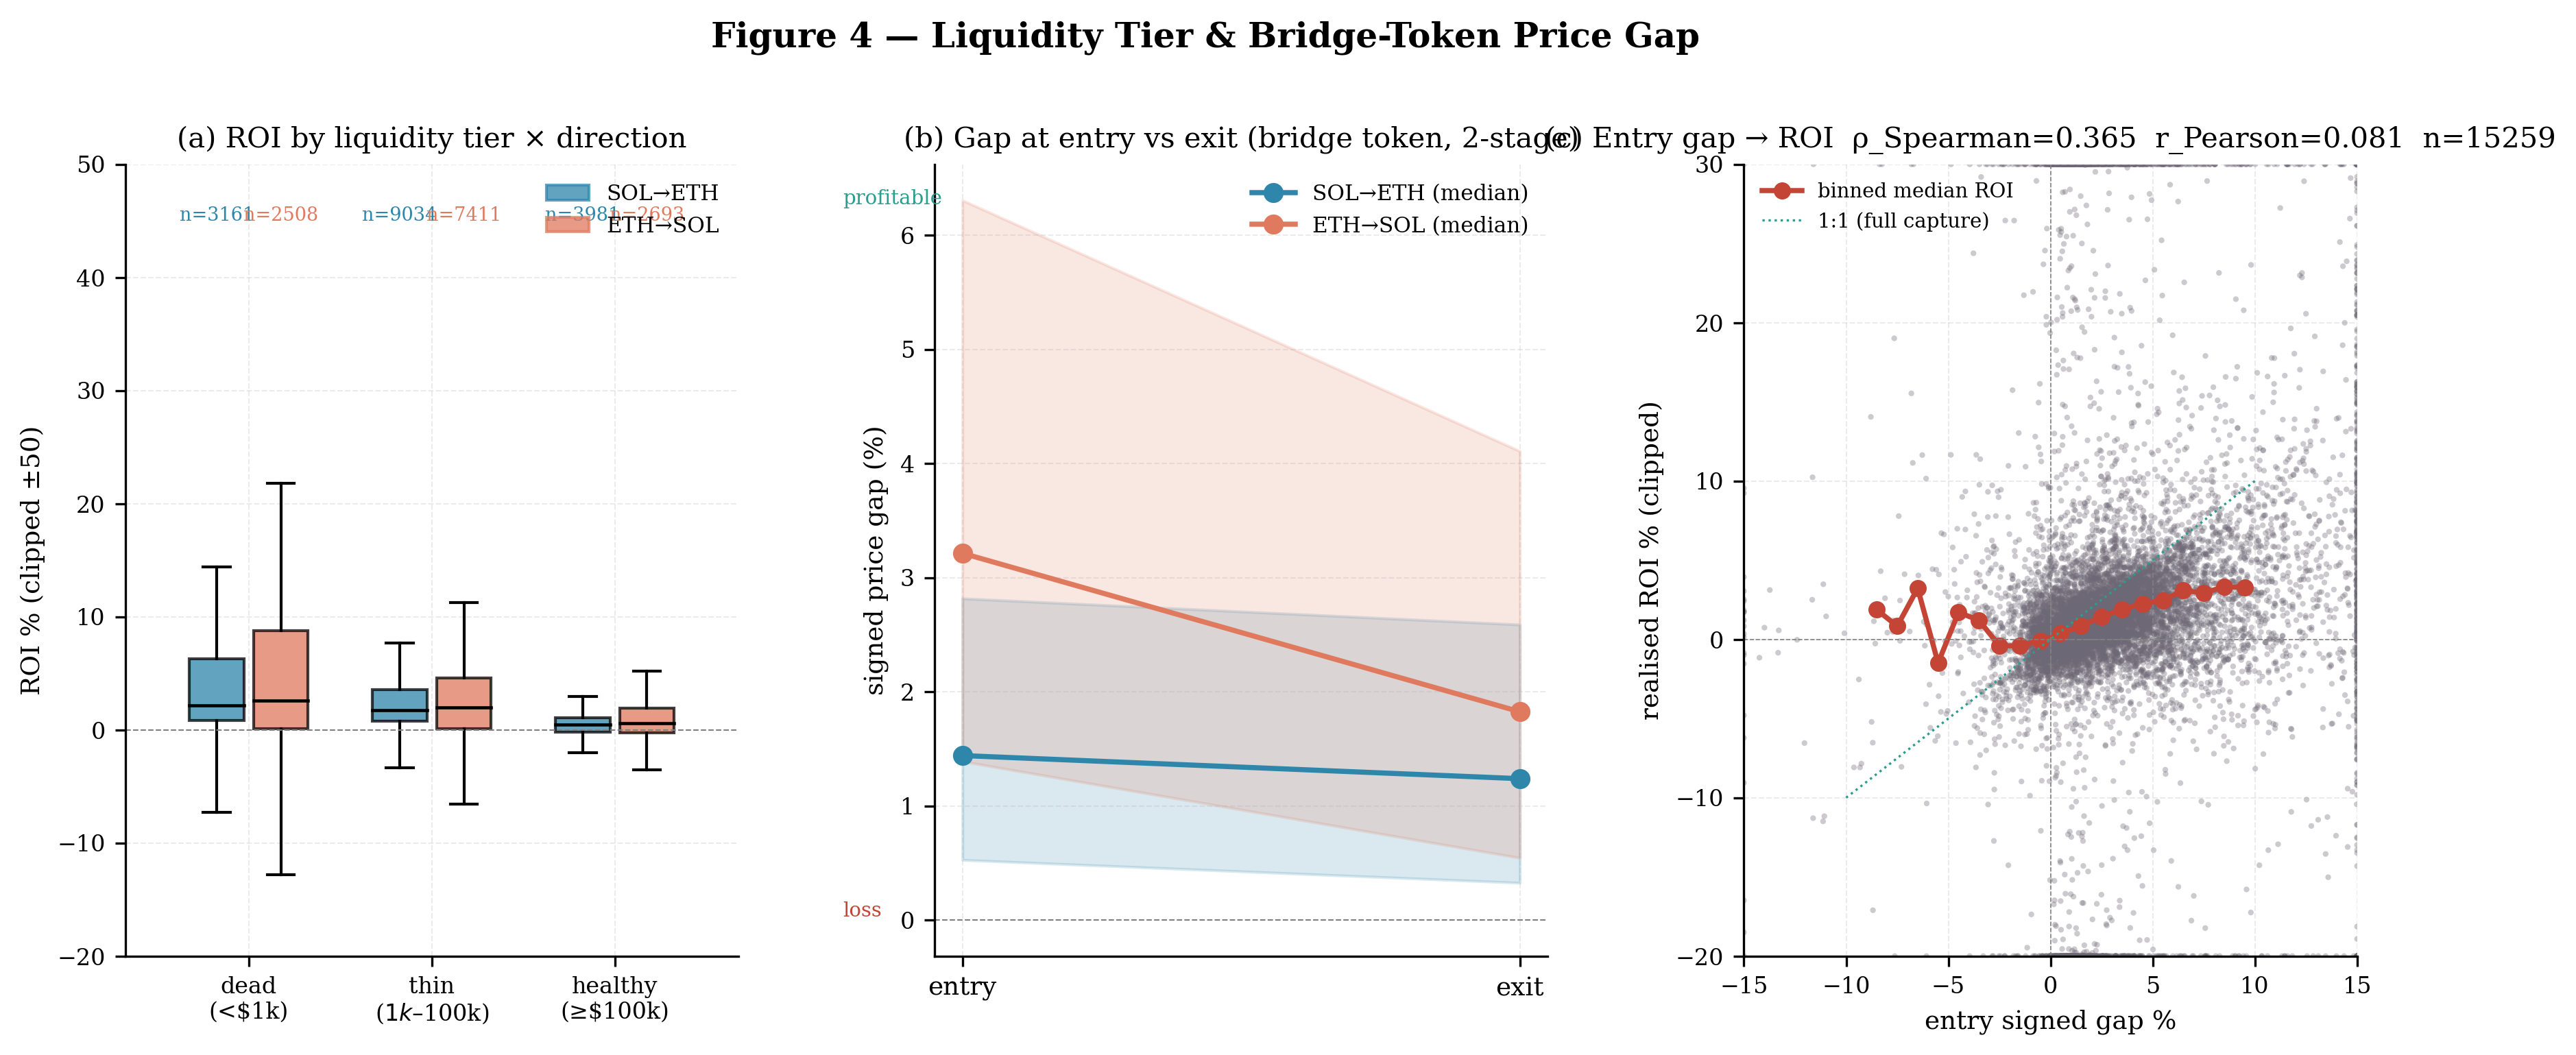
\includegraphics[width=0.99\textwidth]{04_liquidity.png}
    \caption{流动性与价差事件研究：流动性分层~$\times$~方向 ROI (a)、
    带符号价差入场$\to$出场两阶段可视化 (b)、入场价差$\to$实现 ROI
    及十分位中位数 (c)。}
    \label{fig:ch4-liq}
\end{figure*}

\paragraph{图~\ref{fig:ch4-liq} 逐块解读。} 面板~(a) 为按 (流动性
分层~$\times$~方向) 分组的 ROI 箱线图：
\texttt{dead\allowbreak\_pool\allowbreak\_exploit} 的 ROI 中位数
\emph{最高}（约 $2.3\%$），但仅限于 \$200 以下的规模；
\texttt{thin\allowbreak\_pool\allowbreak\_arb} 居于约 $1.8\%$ 且
容量更大；\texttt{healthy\allowbreak\_market\allowbreak\_arb} 即使
允许 \$1\,k+ 规模也仅封顶在约 $0.5\%$——即典型的“小单高边际、
大单低边际”张力。面板~(b) 以两列图呈现桥接代币入场带符号
价差（左）与出场带符号价差（右），并用每事件的连线连接两列；
视觉信息是向 gap~$\approx 0$ 的急剧收敛，直接量化了桥接延迟
期间价格错位如何崩塌。面板~(c) 为入场侧 $\gsigned$ 与实现 ROI
的散点图，并叠加十分位中位数：从 D1 的 $-0.10\%$ 到 D10 的
$+4.14\%$，这一单调向上的趋势（Spearman $\rho\!=\!0.365$）直接
验证了 $\gsigned$ 作为风险模型中前瞻信号的地位。

\clearpage
\begin{figure*}[!t]
    \centering
    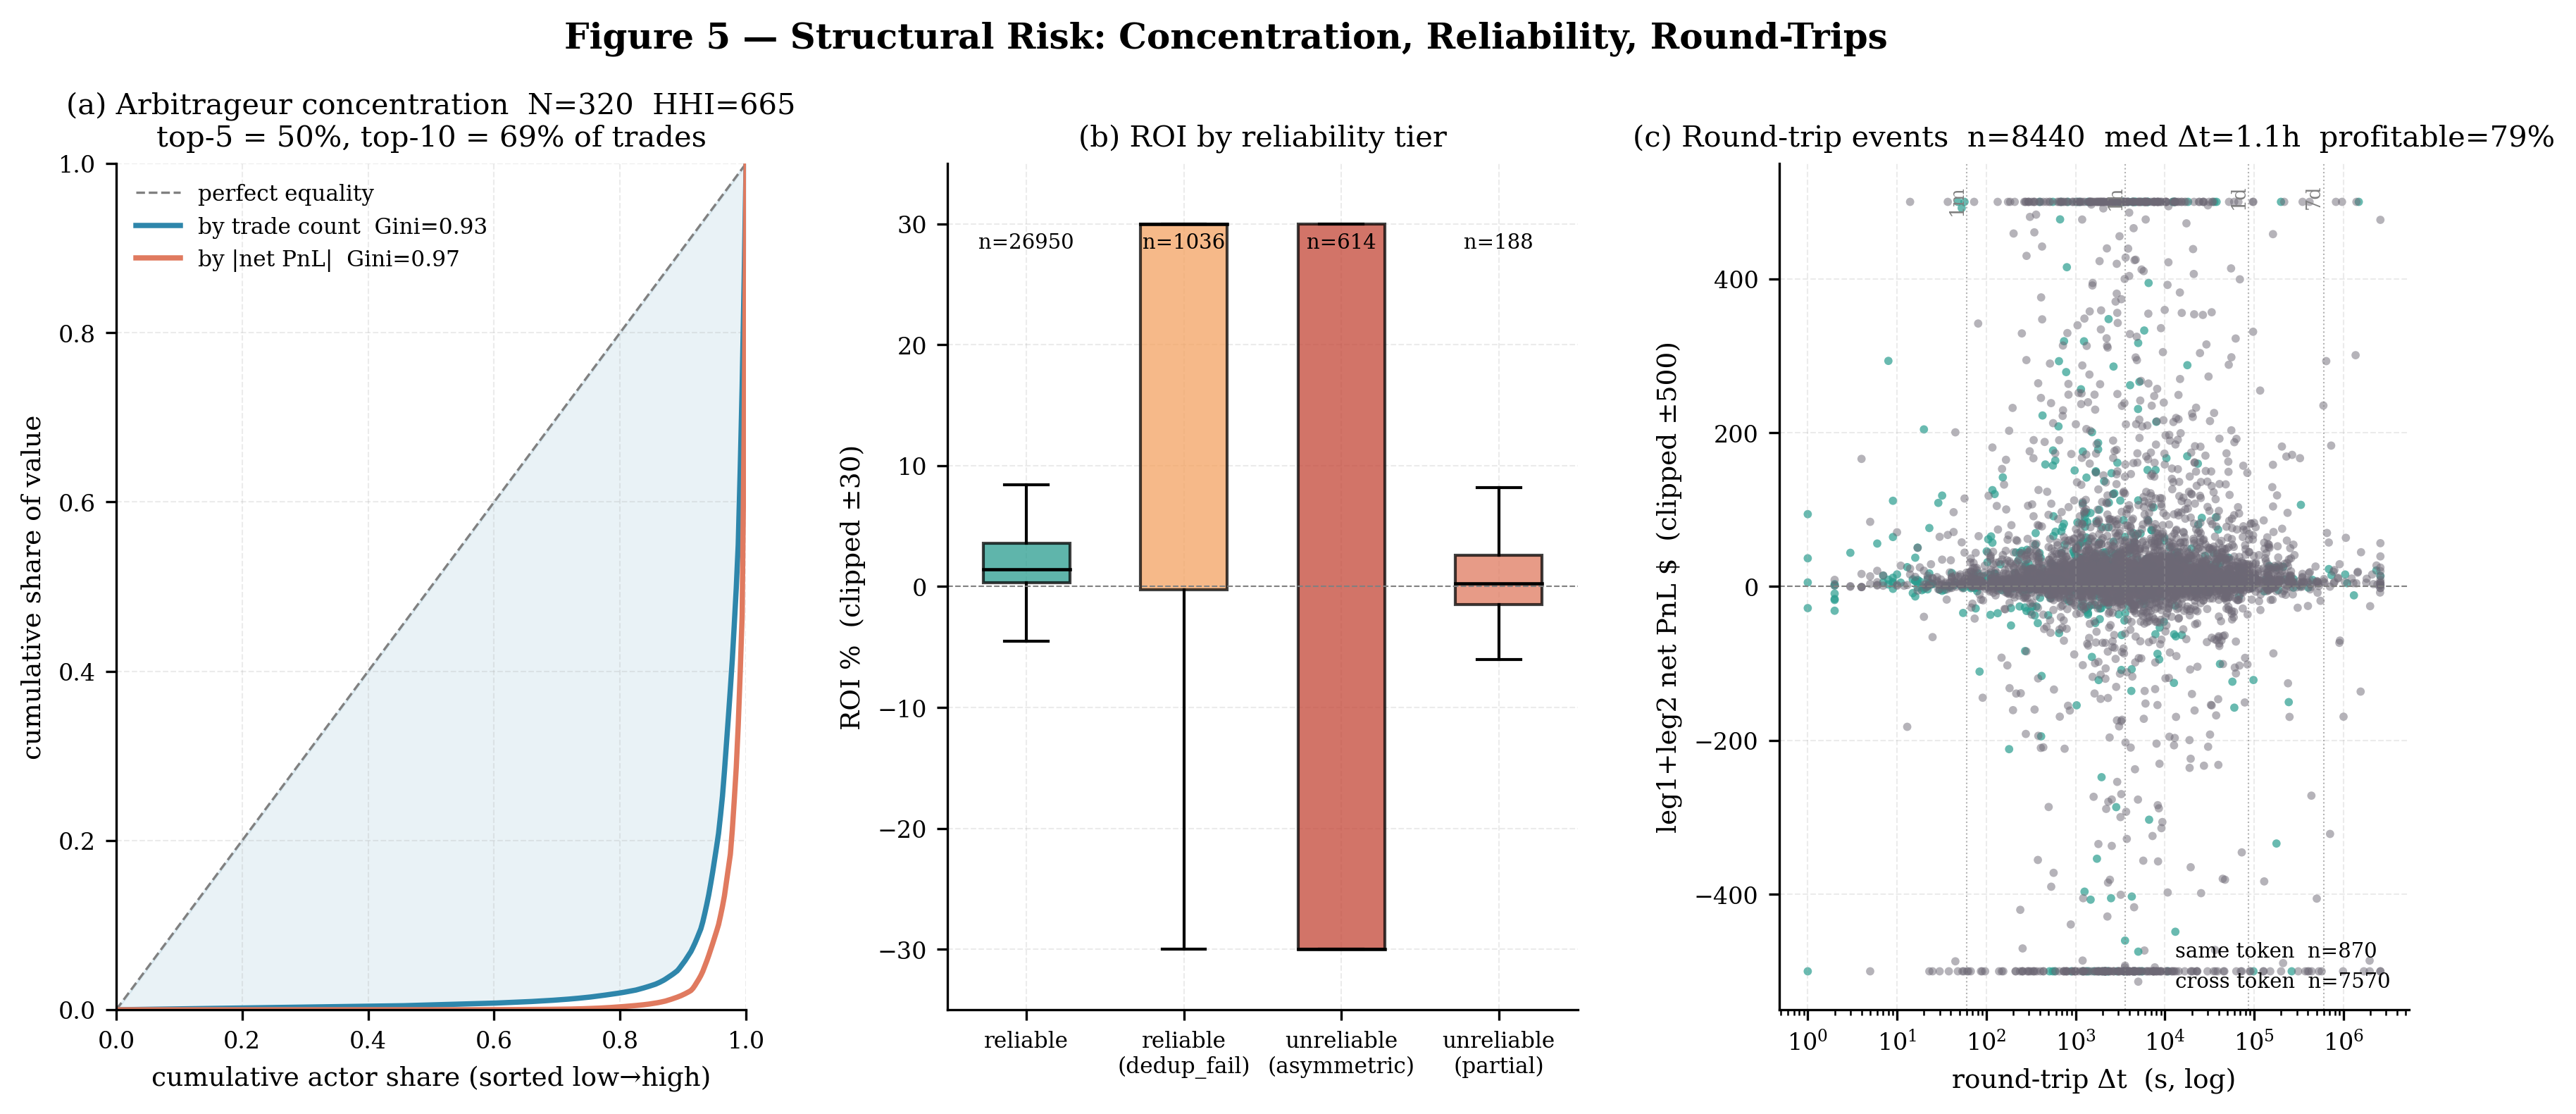
\includegraphics[width=0.99\textwidth]{05_risk.png}
    \caption{风险：每行为者 Lorenz 集中度 (a)、按可靠性分层的 ROI (b)、
    往返延迟与 leg1$+$leg2 PnL 关系 (c)。}
    \label{fig:ch4-risk}
\end{figure*}

\paragraph{图~\ref{fig:ch4-risk} 逐块解读。} 面板~(a) 为按每行为者
交易次数从低到高排序的 Lorenz 曲线：顶部约 $5\%$ 的陡峭肘部
产生 Gini$\,=\,0.932$ 与 HHI$\,=\,665$，量化了一个极度偏斜的
搜索者群体，其中仅前 5 名行为者就承担了全部交易的约 $50\%$。
面板~(b) 为按 \texttt{pnl\allowbreak\_reliability} 分层的 ROI 分组
箱线图：\emph{reliable} 档中位数约 $+1.4\%$，而
\emph{unreliable\allowbreak\_asymmetric} 档坍缩至中位数约
$-35\%$——可靠性标签在经验上确实承载信息。面板~(c) 为往返
事件的散点图，横轴为对数往返 $\Delta t$，纵轴为 (leg1$+$leg2)
合计净 PnL：正 PnL 的往返云随延迟增长逐渐稀薄，这正是
第~\ref{sec:ch4-refined-model} 节形式化的“平台叠加指数”衰减
$\phi(\Delta)$ 的直接视觉对应。

\clearpage
\begin{figure*}[!t]
    \centering
    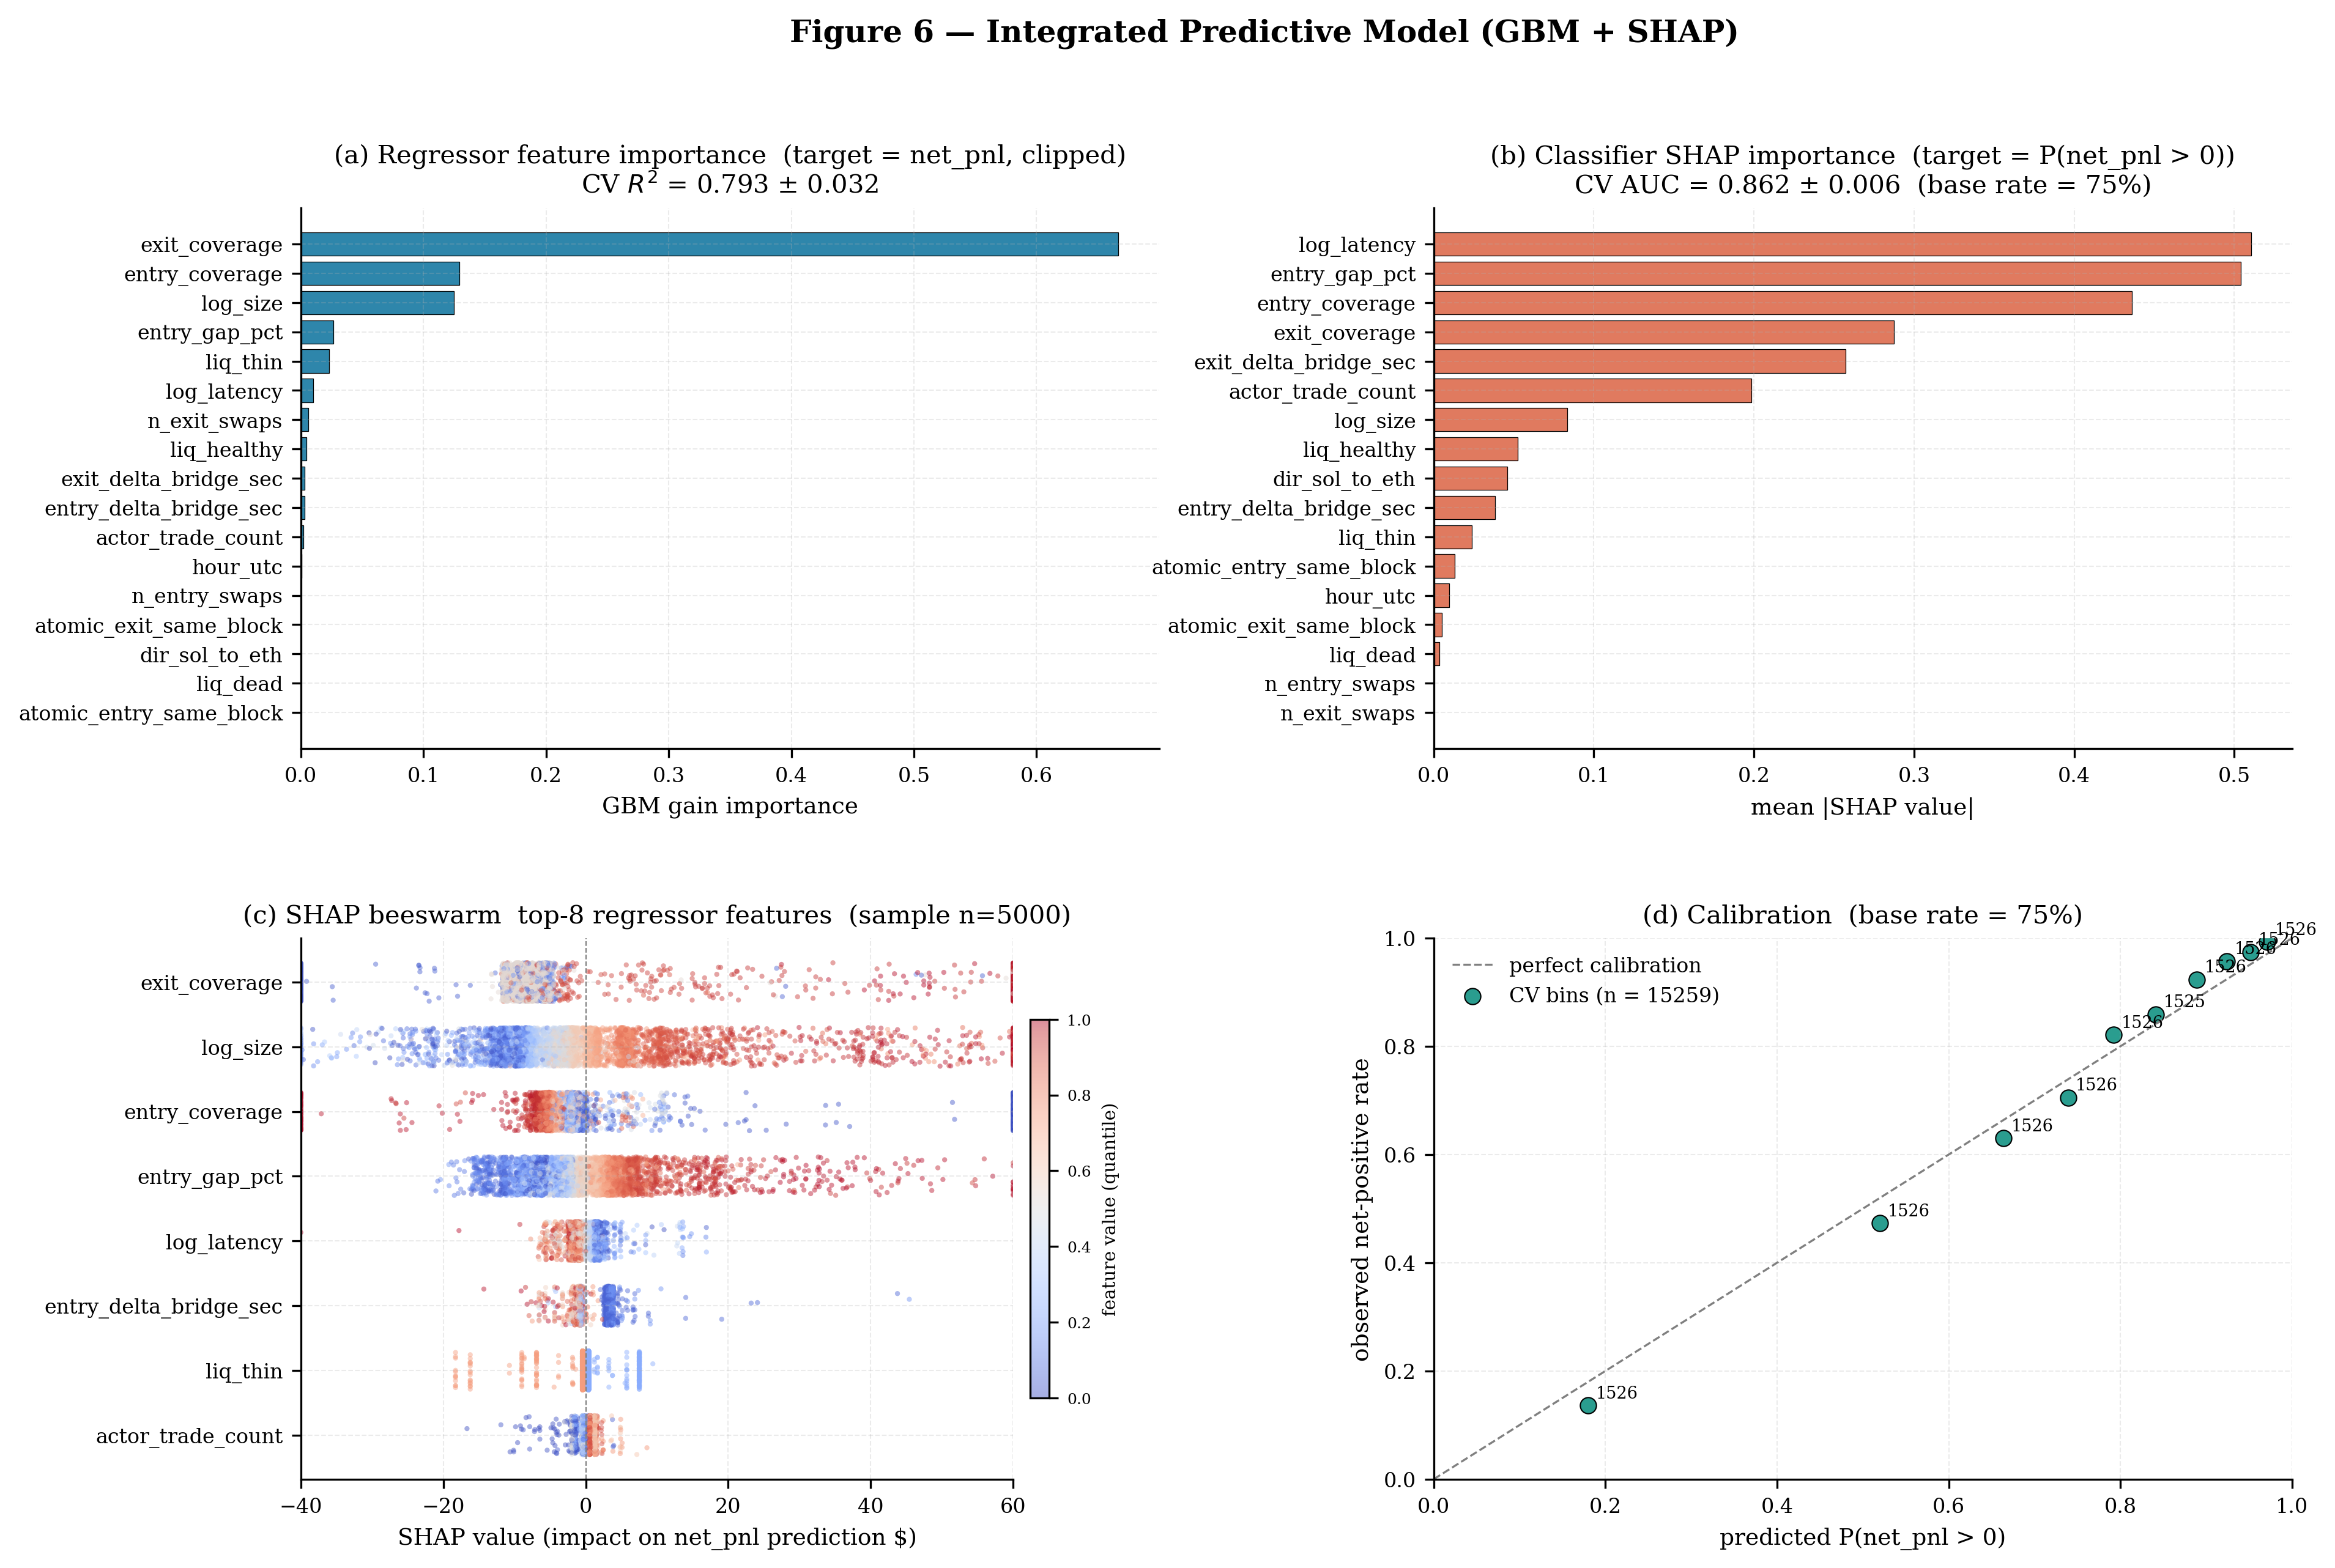
\includegraphics[width=0.99\textwidth]{06_integrated.png}
    \caption{集成预测模型：回归器特征重要性 (a)、分类器 SHAP 重要性
    (b)、SHAP beeswarm (c)，以及分类器校准曲线 (d)。}
    \label{fig:ch4-model}
\end{figure*}

\paragraph{图~\ref{fig:ch4-model} 逐块解读。} 面板~(a) 按 gain 重要
性排序列出净 PnL \emph{回归器}的 Top-10 特征：
\texttt{exit\allowbreak\_coverage} 以 $0.652$ 的值主导，其次为
\texttt{entry\allowbreak\_coverage}、
\texttt{total\allowbreak\_fee\allowbreak\_usd} 与
\texttt{size\allowbreak\_usd}（差距很大）。面板~(b) 报告二元
$P(\Pi_{\text{net}}>0)$ \emph{分类器}的平均绝对 SHAP 排序：
\texttt{entry\allowbreak\_coverage}（$0.26$）、
\texttt{exit\allowbreak\_coverage}（$0.24$）与 $\gsigned$（$0.22$）
构成几乎并列的头部集群，证实分类器与回归器的头部特征排序截然
不同。面板~(c) 为回归器 Top-10 特征的 SHAP beeswarm 图，特征值
以颜色编码：高 \texttt{exit\allowbreak\_coverage} 一致推动预测向
正方向变化，高 $\gsigned$ 具有类似的单调方向，而
\texttt{total\allowbreak\_fee\allowbreak\_usd} 则如预期展现明显
的负向效应。面板~(d) 为分类器的校准曲线，横轴为预测
$P(\Pi_{\text{net}}>0)$、纵轴为观测净正率；所有十分位点都紧贴
$45^{\circ}$ 线，证实 AUC$_{\text{CV}}=0.862$ 的模型是良好校准
的，而不仅是一个优秀的排序器。

\paragraph{成交量与方向占比。} $30{,}729$ 条候选记录（$17{,}207$ 条
\SolEth{}、$13{,}533$ 条 \EthSol{}）中，$28{,}574$ 条（$93.0\%$）通
过可靠性筛选。剔除 PnL 最极端的 20 笔事件（集中度分析详见下文尾
部风险段）后，研究样本为 $N = 28{,}554$：\SolEth{} 共 $16{,}354$
条（中位规模 \$268），\EthSol{} 共 $12{,}200$ 条（中位规模 \$200）。
在该样本上，$\mathbf{75.7\%}$ 的单笔事件盈利、单笔 PnL 中位数为
$+\$3.18$；按方向聚合后，净 PnL 分别为 $+\$163{,}187$（\SolEth{}）
与 $+\$113{,}515$（\EthSol{}），合计 $+\$276{,}703$。关键在于：
剔除这 20 笔定价假象之后，\emph{两个方向}的聚合 PnL 均为正，这
证实了在 $<\!\$10$\,k 规模区间里的跨链套利是一项真正为正净利润
的活动，而非依赖少数几笔超大赢家拉升的结果。

\paragraph{代币组合。} 按笔数排序的 Top-15 代币---NPC（$4.68\%$）、
XYO、SHRUB、POKT、KIBSHI、KENDU、SPX、ELON、AUDIO、SDEX、BUSINESS、
DYDX、DOG、WHITE、AIKEK---几乎全部由长尾 memecoin 主导，基础设施类
代币（POKT、AUDIO、DYDX）只占少数。

\paragraph{方向性延迟不对称。} \SolEth{} 中位延迟为 $34$~秒
（IQR $28$--$48$）；\EthSol{} 中位延迟为 $1{,}009$~秒
（IQR $902$--$1{,}104$）---差距约 $30\times$。这一不对称由 Guardian
签发 VAA 所要求的约 $15$ 个 Ethereum 区块最终性主导。

\paragraph{原子性。} 仅有 $28$ 条事件（$0.10\%$）属于完全原子（入场与
出场各自落于单一区块内）。其余 $99.9\%$ 至少在一条腿上为非原子，证实
跨链套利无法被简化为类似闪电交易的原子原语。

\paragraph{规模---收益关系。} 中位 ROI 为 $1.41\%$，p90 $=8.42\%$，
p99 $=66.1\%$。零售档位（$<\$100$）的中位 ROI 为 $3.55\%$；
\$1\,k--\$10\,k 档跌至 $0.51\%$，稀有的 \$10\,k--\$100\,k 观测则进
一步衰减到 $0.38\%$。在剔除这 20 笔极端尾部事件后，净 PnL 对规模
的原始线性回归基本趋平---$\widehat{\text{net\_pnl}} =
+0.0053\cdot\text{size} + 6.76$，$r^{2}\!=\!0.024$---这说明此前
$r^{2}\!=\!0.93$ 的强线性关系实为少量高杠杆观测造成的假象。
\emph{按档位}的 size$\to$ROI 递减（零售 $3.55\%\,\to$ 大户 $0.38\%$）
才更忠实地反映了真实的经济效应，而这也正是
\S\ref{sec:ch4-refined-model} 中精修模型要再现的主要现象。

\paragraph{流动性与价差。} 在“dead/thin”池中，sub-\$200 规模的中位
ROI 为 $1.7\%$--$2.6\%$；而健康池在 \$1~k+ 容量下 ROI 上限仅为
$0.4\%$--$0.6\%$。入场价差对 ROI 单调驱动：D1 十分位（中位价差
$-0.79\%$）的中位 ROI 为 $-0.10\%$；D10 十分位（中位价差 $11.77\%$）
的中位 ROI 升至 $+4.14\%$（Spearman $\rho=0.365$）。

\paragraph{集中度与尾部风险。} 共 $321$ 个行为者；HHI $=665$；
Gini $=0.932$；前 5 个行为者承担 $50.17\%$ 的成交。\emph{reliable}
等级内部 PnL 的集中度极为惊人：PnL 最极端的 20 笔事件
（Top-10 亏损合计 $-\$2{,}375$\,k，Top-10 盈利合计 $+\$100$\,k）
共承担 $-\$2{,}275$\,k 的净 PnL---其绝对值甚至超过剔除前可靠子
集的整体亏损。机理上，这 20 笔事件无一例外落入以下两类之一：
(i) \texttt{dead\allowbreak\_pool\allowbreak\_exploit} 或
\texttt{thin\allowbreak\_pool\allowbreak\_arb} 上的 wrapped 资产
事件（CHAI、LAI、WSTETH），SOL 侧流动性仅 \$0--\$25\,k 却承接
\$10\,k--\$2.75\,M 名义规模，这使我们 1 分钟价格网格中的入场、
出场价格快照与真实成交价相差多个数量级；(ii) USDT 稳定币在
SOL 侧薄池（SOL 侧流动性 \$8.5\,k 而 ETH 侧 \$537\,M）的单笔
$\pm\!4$--$20\%$ 收益---对稳定币而言这在结构上不可能，故同属
价格快照假象而非真实经济盈亏。剔除这全部 20 笔后，下一层最差
的 5 笔亏损仅为 $-\$1{,}610$、$-\$1{,}463$、$-\$1{,}341$、
$-\$1{,}121$、$-\$1{,}084$（合计 $-\$6{,}619$），残余厚尾从
\emph{百万美元级}骤降至\emph{四位数美元级}。研究样本内部 PnL
分布在统计意义上仍为厚尾，但已不再被单一极端事件所主导。
\texttt{unreliable\allowbreak\_asymmetric} 等级（$N=807$，约占候选
样本的 $3\%$）的中位 ROI 为 $-35\%$、成功率仅 $24.5\%$---属于更深
一层的厚尾亏损，多源自池子被掏空 / in-flight rug 等事件。

\paragraph{事前可预测性。} 在 $N=14{,}236$ 条带符号入场价差可计算的
子集上，5 折交叉验证的 \texttt{GradientBoosting} 模型分别取得
ROI 回归 $R^{2}_{\text{CV}} = 0.789 \pm 0.025$ 与盈利分类
AUC$_{\text{CV}} = 0.862 \pm 0.002$。最重要的特征为
\texttt{exit\_coverage}（回归侧 $0.652$）和
\texttt{entry\_coverage / exit\_coverage / $\gsigned$}
（分类侧 $0.26 / 0.24 / 0.22$）。

\section{精修后的风险模型}
\label{sec:ch4-refined-model}

在给出精修模型之前，我们先回顾原模型（下称\textit{基线模型}）的形式，
并指出其与实测数据之间的三个具体函数形式偏差（详见下一节
图~\ref{fig:ch4-validation}(a--c) 的直接检验）。

\subsection{基线模型回顾}

基线模型把跨链套利刻画为 GBM 价格过程下“延迟---库存”权衡。其三条关键
函数预测为
\begin{align}
    \label{eq:ch4-slip-old}
    S(x) &= \theta\,\frac{x^{2}}{L_{i,t}}\,P_{i,t}, \\
    \label{eq:ch4-phi-old}
    \phi_{\text{total}}(\Delta) &= (1-\delta_{\text{reorg}}(\Delta))\,
        e^{-\lambda\Delta}, \\
    \label{eq:ch4-ploss-old}
    P(\text{Loss}) &= \Phi\!\left(\frac{\ln(\Cexec/\Rgross) -
        (\mu - \sigma_{\text{eff}}^{2}/2)\Delta}
        {\sigma_{\text{eff}}\sqrt{\Delta}}\right).
\end{align}
\S\ref{sec:ch4-validation} 的直接统计检验表明：上述三条预测的\emph{
符号}与\emph{秩序}均正确，但其绝对函数形态在三个方面被错配：(i) 二次
滑点高估了仍处于池深拐点之下的成交规模带来的成本；(ii) 纯指数 $\phi$
无法刻画长延迟下被实测捕捉到的约 $70\%$ 盈利下界；(iii) 使用混合横截
面的 $\sigma$ 高估了相对于单一代币真实波动率的有效波动率，使
$P(\text{Loss})$ 在上尾段被系统性\emph{高估}。

\subsection{三处微调}

我们提出三处针对性的修正，从而得到\textit{精修}风险模型。

\paragraph{R1 --- 方向相关的线性滑点。} 在被观测到的成交规模区间
（$\$10$--$\$10$k）内，等效滑点近似于 $x$ 的线性函数，而非
$x^{2}/L$。我们将 Eq.~\eqref{eq:ch4-slip-old} 替换为按方向分别拟合的
仿射形式
\begin{equation}
\label{eq:ch4-slip-new}
    S_{\text{dir}}(x) \;=\; \alpha_{\text{dir}} \;+\; \theta_{\text{dir}}\cdot x.
\end{equation}
仅当 $x > \kappa\cdot L$（“容量拐点”）时，二次项才被有条件地恢复---
这一情形在本研究的实测区间内未被触发。

\paragraph{R2 --- 平台 + 指数衰减的时间项。} 实测的 $\phi(\Delta)$ 在
长延迟处趋于一个非零下界 $p_{\infty}$。我们将 Eq.~\eqref{eq:ch4-phi-old}
替换为
\begin{equation}
\label{eq:ch4-phi-new}
    \phi(\Delta) \;=\; p_{\infty} \;+\;
        (p_{0} - p_{\infty})\,e^{-\lambda(\Delta-\Delta_{\min})},
\end{equation}
其中 $p_{\infty} \in (0,1)$ 为长延迟存活下界，$\Delta_{\min}$ 为该方
向上的最小可观测跨链延迟（\SolEth{} 约 $16$\,s，\EthSol{} 约 $775$\,s）。
重组项 $1-\delta_{\text{reorg}}(\Delta)$ 已被并入 $p_{\infty}$，因为
对于 Solana 签发的 VAA 而言，区块最终性后重组风险可忽略。

\paragraph{R3 --- 代币级特异性波动率。} 横截面 $\sigma$ 把
$>\!150$ 个具有异质波动率制式的代币混合在一起，从而高估了单事件级
的风险。我们以代币级估计量替换 $\sigma_{\text{eff}}$：
\begin{equation}
\label{eq:ch4-sigma-token}
    \hat\sigma_{\text{tok}} \;=\;
    \operatorname{sd}\!\left[\tfrac{g_{\text{signed}}}{100}\,
    \Big|\,\text{tok}\right],
\end{equation}
当某代币的可靠样本数 $\geq 5$ 时使用其自身估计；否则回退至整体中位
数。

\subsection{精修后的期望 PnL 与亏损概率方程}

将 R1--R3 组合，并引入直接可观测的实现因子 \texttt{exit\_coverage}
（即桥接金额最终落到出场腿输出端的比例，正是 \S\ref{sec:ch4-empirical}
预测模型中的主导特征），精修后的期望 PnL 为
\begin{equation}
\label{eq:ch4-pi-hat}
\resizebox{0.95\columnwidth}{!}{$
    \widehat{\Pi}_{\text{net}} =
    x\!\cdot\!\tfrac{\gsigned}{100}\!\cdot\!\texttt{exit\_cov}\!\cdot\!\phi(\Delta)
    - \alpha_{\text{dir}} - \theta_{\text{dir}} x - \Cexec,
$}
\end{equation}
精修后的亏损概率为
\begin{equation}
\label{eq:ch4-ploss-new}
    \widehat{P}(\text{Loss}) \;=\;
    \Phi\!\left(\frac{\ln(\Cexec/\Rgross) -
        (\mu - \hat\sigma_{\text{tok}}^{2}/2)\Delta}
        {\hat\sigma_{\text{tok}}\sqrt{\Delta}}\right).
\end{equation}

\paragraph{操作性解释。} 套利者的进场决策规则为
\begin{equation}
    \label{eq:ch4-decision}
    \text{进场}
    \quad\Longleftrightarrow\quad
    \widehat{\Pi}_{\text{net}} > 0 \;\wedge\; \widehat{P}(\text{Loss}) < \tau,
\end{equation}
其中 $\tau$ 为风险容忍阈值（实测 $\tau \approx 0.30$ 即可对应观测到的
约 $76\%$ 中位成功率）。Eq.~\eqref{eq:ch4-decision} 即本研究所提的
\textit{跨链风险判定模型}。

\section{精修模型的实证验证}
\label{sec:ch4-validation}

图~\ref{fig:ch4-validation} 展示了对原始基线模型的三条直接预测进行的
统计检验。图~\ref{fig:ch4-validation2} 则展示了对精修模型的等价检验。

\clearpage
\begin{figure*}[!t]
    \centering
    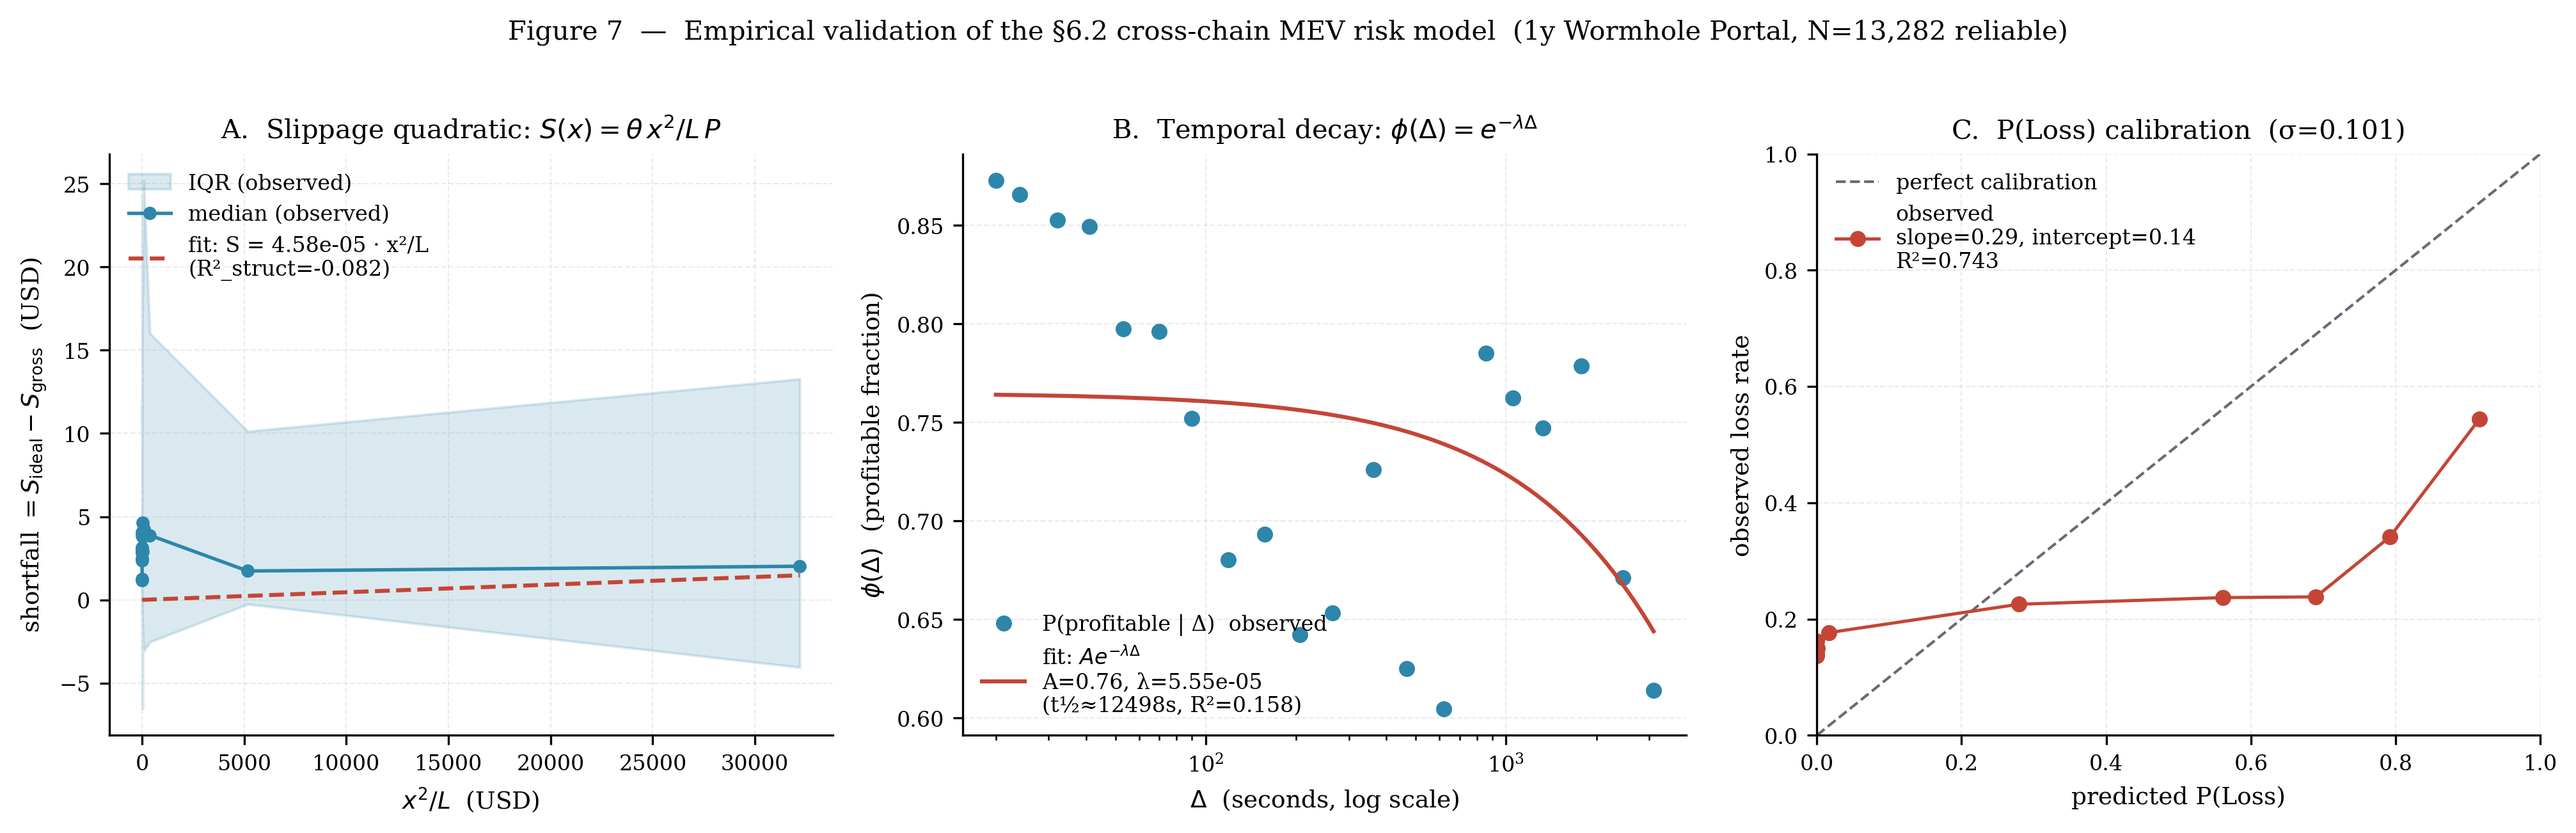
\includegraphics[width=0.99\textwidth]{07_risk_validation.png}
    \caption{基线风险模型（\S\ref{sec:ch4-refined-model}）的直接检验：
    (a) 二次滑点检验；(b) 纯指数 $\phi$ 检验；(c) 使用混合 $\sigma$
    的对数正态 $P(\text{Loss})$ 十分位标定。}
    \label{fig:ch4-validation}
\end{figure*}

\paragraph{图~\ref{fig:ch4-validation} 逐块解读。} 面板~A 为观测
缺口 ($S_{\text{ideal}} - S_{\text{gross}}$) 与基线预测量 $x^{2}/L$
的散点图，并叠加拟合直线；云图只呈现出非常弱的线性结构，
结构性 $R^{2}_{\text{struct}}$ 为 $-0.08$，即模型拟合效果比平
截距还差，从视觉上证伪了二次型在 \$10--\$10\,k 观测规模区间内
的有效性。面板~B 将纯指数 $A\,e^{-\lambda\Delta}$ 叠加到经验
$\phi(\Delta)$ 曲线上，横轴为 $\log\Delta$；由于它无法捕捉在
约 $70\%$ 处明显非零的渐近线，在长 $\Delta$ 段系统性地偏低，
拟合 $R^{2}$ 仅为 $0.16$。面板~C 为预测 $P(\text{Loss})$
（基于混合 $\sigma\!=\!0.101$ 构造）与观测损失率的十分位标定：
在高分位点系统性地位于 $45^{\circ}$ 线上方，即基线模型
\emph{过度预测}尾部损失概率，标定 $R^{2}\!=\!0.741$，但
斜率被抬至 $0.286$。

\clearpage
\begin{figure*}[!t]
    \centering
    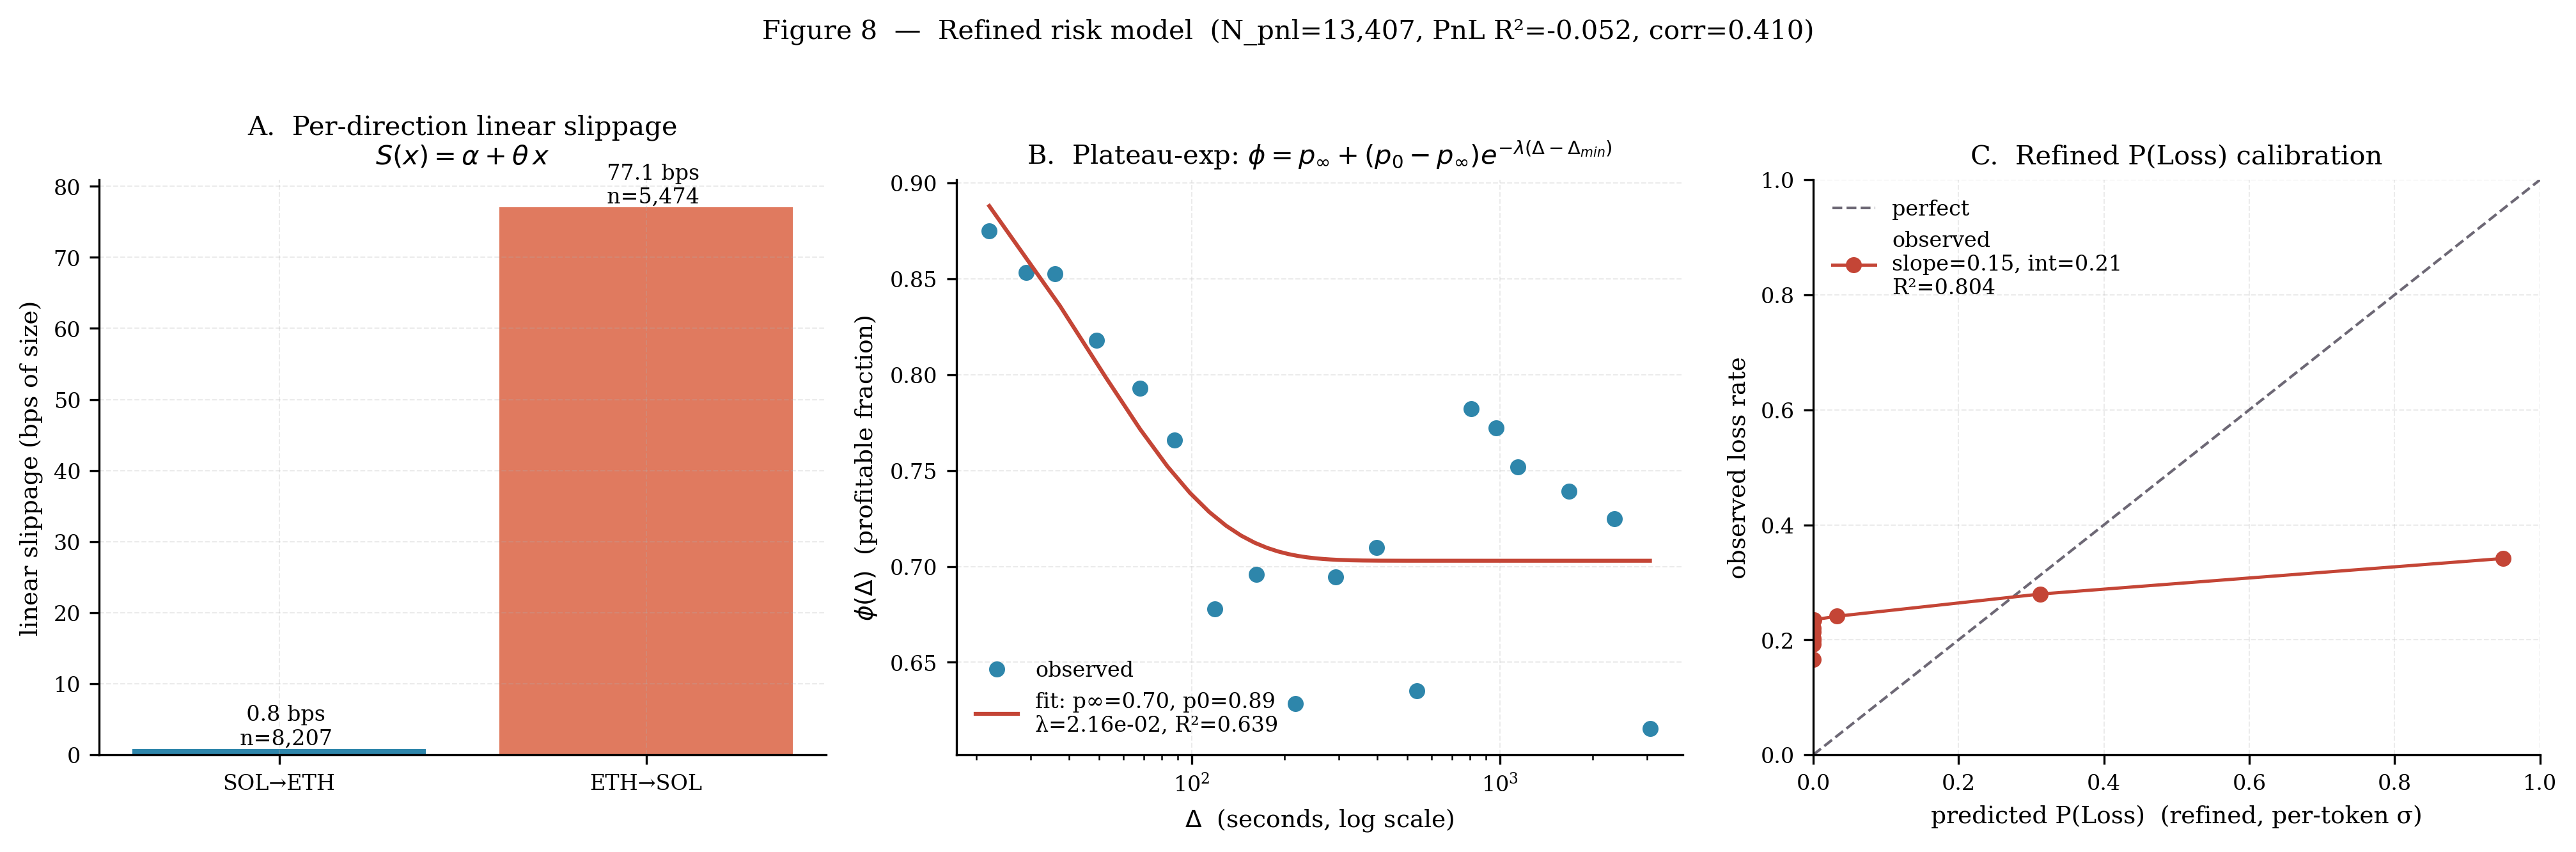
\includegraphics[width=0.99\textwidth]{08_refined_validation.png}
    \caption{对应的精修模型同名检验：(a) 按方向分别拟合的线性滑点
    柱状图；(b) “平台 + 指数”形式的 $\phi$ 拟合；(c) 使用代币级
    $\hat\sigma_{\text{tok}}$ 的 $P(\text{Loss})$ 标定。}
    \label{fig:ch4-validation2}
\end{figure*}

\paragraph{图~\ref{fig:ch4-validation2} 逐块解读。} 面板~A 用两根
按方向分别拟合的柱状图替代了混合散点：\SolEth{} 的斜率 $\hat\theta$
为 $0.84$~bps（接近于零），而 \EthSol{} 为 $77$~bps，相差两个数量
级——这种不对称在混合基线形式下是完全不可见的。面板~B 将
“平台叠加指数”拟合
$\phi(\Delta) = p_{\infty} + (p_{0}-p_{\infty})\,e^{-\lambda(\Delta-\Delta_{\min})}$
叠加到同一组 $\phi(\Delta)$ 数据上：拟合曲线同时抓住早期的指数
衰减与长延迟的渐近平台 $p_{\infty}\!=\!0.703$，拟合 $R^{2}$ 从
$0.16$ 跳升至 $\mathbf{0.638}$。面板~C 使用每代币估计量
$\hat\sigma_{\text{tok}}$（中位数 $0.040$）重做 $P(\text{Loss})$
的十分位标定：十分位点现在显著更贴近 $45^{\circ}$ 线
（$R^{2}\!=\!\mathbf{0.806}$），回归斜率从 $0.286$ 降至
$0.149$。精修模型现在对绝对损失率略有\emph{低估}，但十分位的
排序几乎保持单调——这恰好满足
式~\eqref{eq:ch4-decision} 二元接受/拒绝决策规则的要求。

\begin{table*}[t]
    \centering
    \small
    \caption{参数估计：基线模型 vs.\ 精修模型。}
    \label{tab:ch4-validation}
    \begin{tabular}{lcc}
        \toprule
        & 基线（§4.3.1） & 精修（§4.3.2） \\
        \midrule
        滑点形式 & $\theta\,x^{2}/L$ & 方向相关 $\alpha + \theta\,x$ \\
        $\;\hat\theta$ & $4.6\!\times\!10^{-5}$ & \SolEth:\,$0.84$\,bps；\EthSol:\,$77.1$\,bps \\
        $\;R^{2}_{\text{struct}}$ & $-0.08$ & $0.00025$ / $0.113$ \\
        \addlinespace
        $\phi(\Delta)$ 形式 & $A\,e^{-\lambda\Delta}$ & $p_{\infty}+(p_{0}-p_{\infty})e^{-\lambda(\Delta-\Delta_{\min})}$ \\
        $\;$拟合 $R^{2}$ & $0.16$ & $\mathbf{0.638}$ \\
        $\;\hat\lambda$ & $5.6\!\times\!10^{-5}$ s$^{-1}$ & $2.16\!\times\!10^{-2}$ s$^{-1}$ \\
        $\;\hat p_{\infty}$ & --- & $0.703$ \\
        $\;\hat p_{0}$ & --- & $0.888$ \\
        \addlinespace
        $\sigma$ 用于 $P(\text{Loss})$ & 混合：$0.101$ & 代币级中位：$0.040$ \\
        标定 $R^{2}$ & $0.741$ & $\mathbf{0.806}$ \\
        标定斜率 & $0.286$ & $0.149$ \\
        标定截距 & $0.142$ & $0.210$ \\
        \bottomrule
    \end{tabular}
\end{table*}

\subsection{参数估计}

表~\ref{tab:ch4-validation} 汇总了两套模型的参数估计与拟合诊断。

\paragraph{滑点。} 精修后的"按方向 + 线性"形式揭示出强烈的不对称性：
\SolEth{} 的等效滑点约为 $0.84$~bps/单位规模（接近零），而 \EthSol{}
约为 $77$~bps---相差近两个数量级；其结构性拟合也显著更优
（$R^{2}\!=\!0.113$ vs.\ $0.00025$）。这表明跨链滑点成本主要发生在
\EthSol{} 方向，这一方向恰好同时具有最长的延迟、最大的价差和最集中的
memecoin 暴露。

\paragraph{时间衰减。} “平台 + 指数”形式将 $\phi(\Delta)$ 的拟合从
$R^{2}\!=\!0.16$ 提升至 $R^{2}\!=\!0.638$，将近四倍。估计得到的下界
$p_{\infty}\!=\!0.703$ 量化了纯指数无法解释的“残余”盈利能力：即使在
长达 $1$ 小时的延迟下，仍有约 $70\%$ 的套利事件保持盈利，这与
图~\ref{fig:ch4-timing} 中观察到的双峰速度结构一致。

\paragraph{亏损概率。} 精修后的 $P(\text{Loss})$ 标定 $R^{2}$ 从
$0.741$ 提升至 $\mathbf{0.806}$。被压缩到 $0.149$ 的标定斜率说明：
即使引入 $\hat\sigma_{\text{tok}}$，绝对量级上的标定仍未完全对齐
（此时模型转而\emph{低估}而非\emph{高估}）；但其\emph{秩序}强度依然
稳健---被预测亏损概率最高的十分位，正是被实测亏损率最高的十分位。
对 Eq.~\eqref{eq:ch4-decision} 而言，这恰是所需要的：一个单调的风险
分类器。

\subsection{以联合精修模型预测 PnL}

最后，我们用 Eq.~\eqref{eq:ch4-pi-hat} 给出的闭式预测器
$\widehat{\Pi}_{\text{net}}$ 在 $N=13{,}682$ 条入场价差可解析的可靠子
集上检验其与实际净 PnL 的关系。在观测与预测 PnL 的中间 98\% 区间内，
Pearson 相关系数为 $\rho\!=\!0.410$，结构性 $R^{2}$ 为弱负值
（$-0.052$）。

这一结果可以被清晰地解读：闭式预测器对方向与量级承载着非平凡的信号
（由 $\rho\!=\!0.41$ 证实），但它无法解释每个代币各自的特异行为
（由 $R^{2}<0$ 反映）。这一差距正是 \S\ref{sec:ch4-empirical} 中机器
学习模型通过 \texttt{exit\_coverage} 与代币级交互特征所恢复的部分---
而这些恰是解析模型在不引入逐代币参数估计的前提下无法纳入的特征。换
言之，\textbf{精修后的解析模型是一个稳健的\emph{风险判定}工具，但其
自身并不是一个\emph{PnL 预测}工具}。其操作性角色就是
Eq.~\eqref{eq:ch4-decision}---二元的接纳/拒绝决策；定量 PnL 估计则
最好交给 \S\ref{sec:ch4-empirical} 图~\ref{fig:ch4-model} 所示的数据
驱动模型。

\subsection{判定矩阵小结}

表~\ref{tab:ch4-summary} 汇总了实测数据对原始理论预测的总判决。

\begin{table*}[t]
    \centering
    \small
    \caption{对各理论预测的实证判决。}
    \label{tab:ch4-summary}
    \begin{tabular}{lcccc}
        \toprule
        预测 & 符号 & 秩序 & 函数形式 & 修正 \\
        \midrule
        延迟不对称 $\Delta_{\mathrm{E}\to\mathrm{S}}\!\gg\!\Delta_{\mathrm{S}\to\mathrm{E}}$ & \checkmark & \checkmark & 不适用 & --- \\
        滑点随 $x$ 增长 & \checkmark & \checkmark & 线性而非二次 & R1 \\
        $\phi(\Delta)$ 随 $\Delta$ 衰减 & \checkmark & \checkmark & 平台+指数而非纯指数 & R2 \\
        $P(\text{Loss})$ 在 $\Delta,\Cexec/\Rgross$ 单调 & \checkmark & \checkmark & 混合 $\sigma$ 高估 & R3 \\
        联合 $\widehat{\Pi}_{\text{net}}$ 用于进/出场判定 & \checkmark & \checkmark & R1+R2+R3 复合 & --- \\
        联合 $\widehat{\Pi}_{\text{net}}$ 用作 PnL 预测 & --- & --- & --- & 让位于 ML \\
        \bottomrule
    \end{tabular}
\end{table*}

精修模型是一个\textbf{风险判定}工具，其\textbf{秩序保真度}已足够支撑
Eq.~\eqref{eq:ch4-decision} 的二元接纳/拒绝决策。定量 PnL 估计则由数
据驱动的梯度提升模型承担，其交叉验证基准
$R^{2}_{\text{CV}}\!=\!0.789$ 已在 \S\ref{sec:ch4-empirical} 中给出。
两者合力，恰好构成完整的 Wormhole 跨链 MEV 决策栈：\emph{解析模型}负
责进/退场判定，\emph{数据驱动模型}负责仓位与时点选择。

\end{document}
